\documentclass[a4j,11pt,oneside,openany,report]{jsbook}

\usepackage{comment}
\usepackage[a4paper,truedimen,margin=25truemm]{geometry}
\usepackage{cscover}
\usepackage[dvipdfmx]{graphicx}
\usepackage[nobreak]{cite}
\usepackage[a4paper,dvipdfmx,pdfdisplaydoctitle=true,%
    bookmarks=true,bookmarksnumbered=true,bookmarkstype=toc,bookmarksopen=true,%
    pdftitle={全天周ビデオ通信端末を用いた非対称型コミュニケーションに関する研究},%
    pdfauthor={栗岡 保}%
    ]{hyperref}
\usepackage{pxjahyper}

\renewcommand{\bibname}{参考文献}
\setcounter{tocdepth}{2}
\pagestyle{plain}

\newcommand{\TODO}[1]{\textbf{[TODO: #1]}}
%\renewcommand{\TODO}[1]{}

\thesistype{学士特定課題研究論文}
\title{全天周ビデオ通信端末を用いた非対称型コミュニケーションに関する研究}
\author{栗岡 保}
\studentid{17B05518}
\affiliation{東京工業大学\\情報理工学院\\情報工学系} 
\date{2021年1月}

\supervisorname{指導教員}
\supervisor{小池 英樹}
%\dsupervisorname{副指導教員}
%\dsupervisor{工学 次郎}

\begin{document}

\frontmatter
\maketitle

\chapter{概要}
学士特定課題研究論文は、シングルカラムでページ数に制限はない。

\tableofcontents
\listoffigures
\listoftables

%%%%%%%%%%%%%%%%%%%%%%%%%%%%%%%%%%%%%%%%%%%%%%%%%%

\mainmatter
\chapter{序論}

\section{本研究の背景} 本章では、本研究の背景、目的、本論文の構成について述べる。
\section{本研究の目的}近年、様々なビデオ会議アプリケーション(図\ref{fig:1})が登場している。
その例としては、zoom\cite{1}やGoogle Meet\cite{2}が挙げられる。
新型コロナウイルス感染症の流行により、ビデオ会議の需要がさらに高まりつつある。
\begin{figure}[tb]
  \centering
  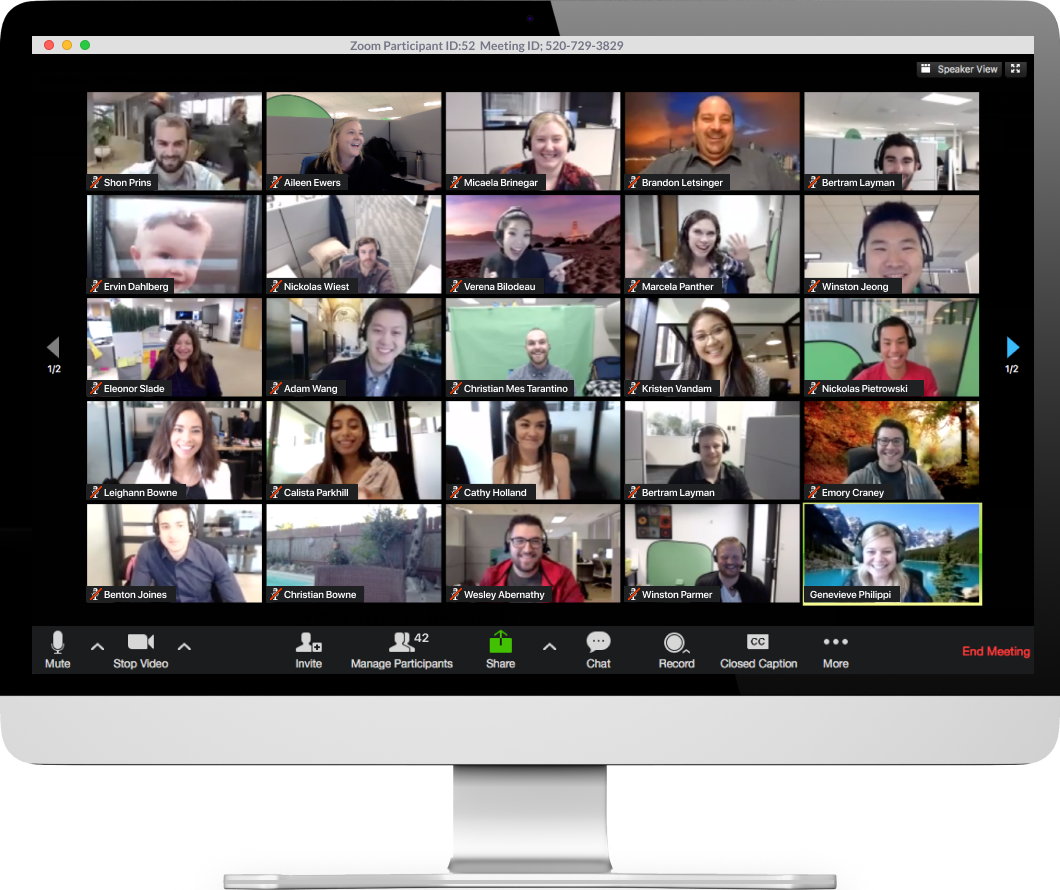
\includegraphics[scale=0.5]{fig/zoom-monitor-screen.png}
  \caption{zoom}\label{fig:1}\cite{1}
\end{figure}

しかし、ビデオ会議における様々な問題点も指摘されている。
例えばRoel\cite{3}は、カメラの視覚外の情報や、人物の情報の不足のために、対面時のような
インタラクションを得られないことを指摘している。

一方で、昨今は誰でも気軽に全天球映像(図\ref{fig:2})を撮影することができるようになっている。
その例として、全天球カメラ(360度カメラ,全天周カメラ,全方位カメラなどともいう (図\ref{fig:3}))
を使用して、全天球映像をヘッドマウントディスプレイを用いて観覧したり、パノラマ映像として動画や静止画を
保存することが出来るようになっている。
\begin{figure}[tb]
  \centering
  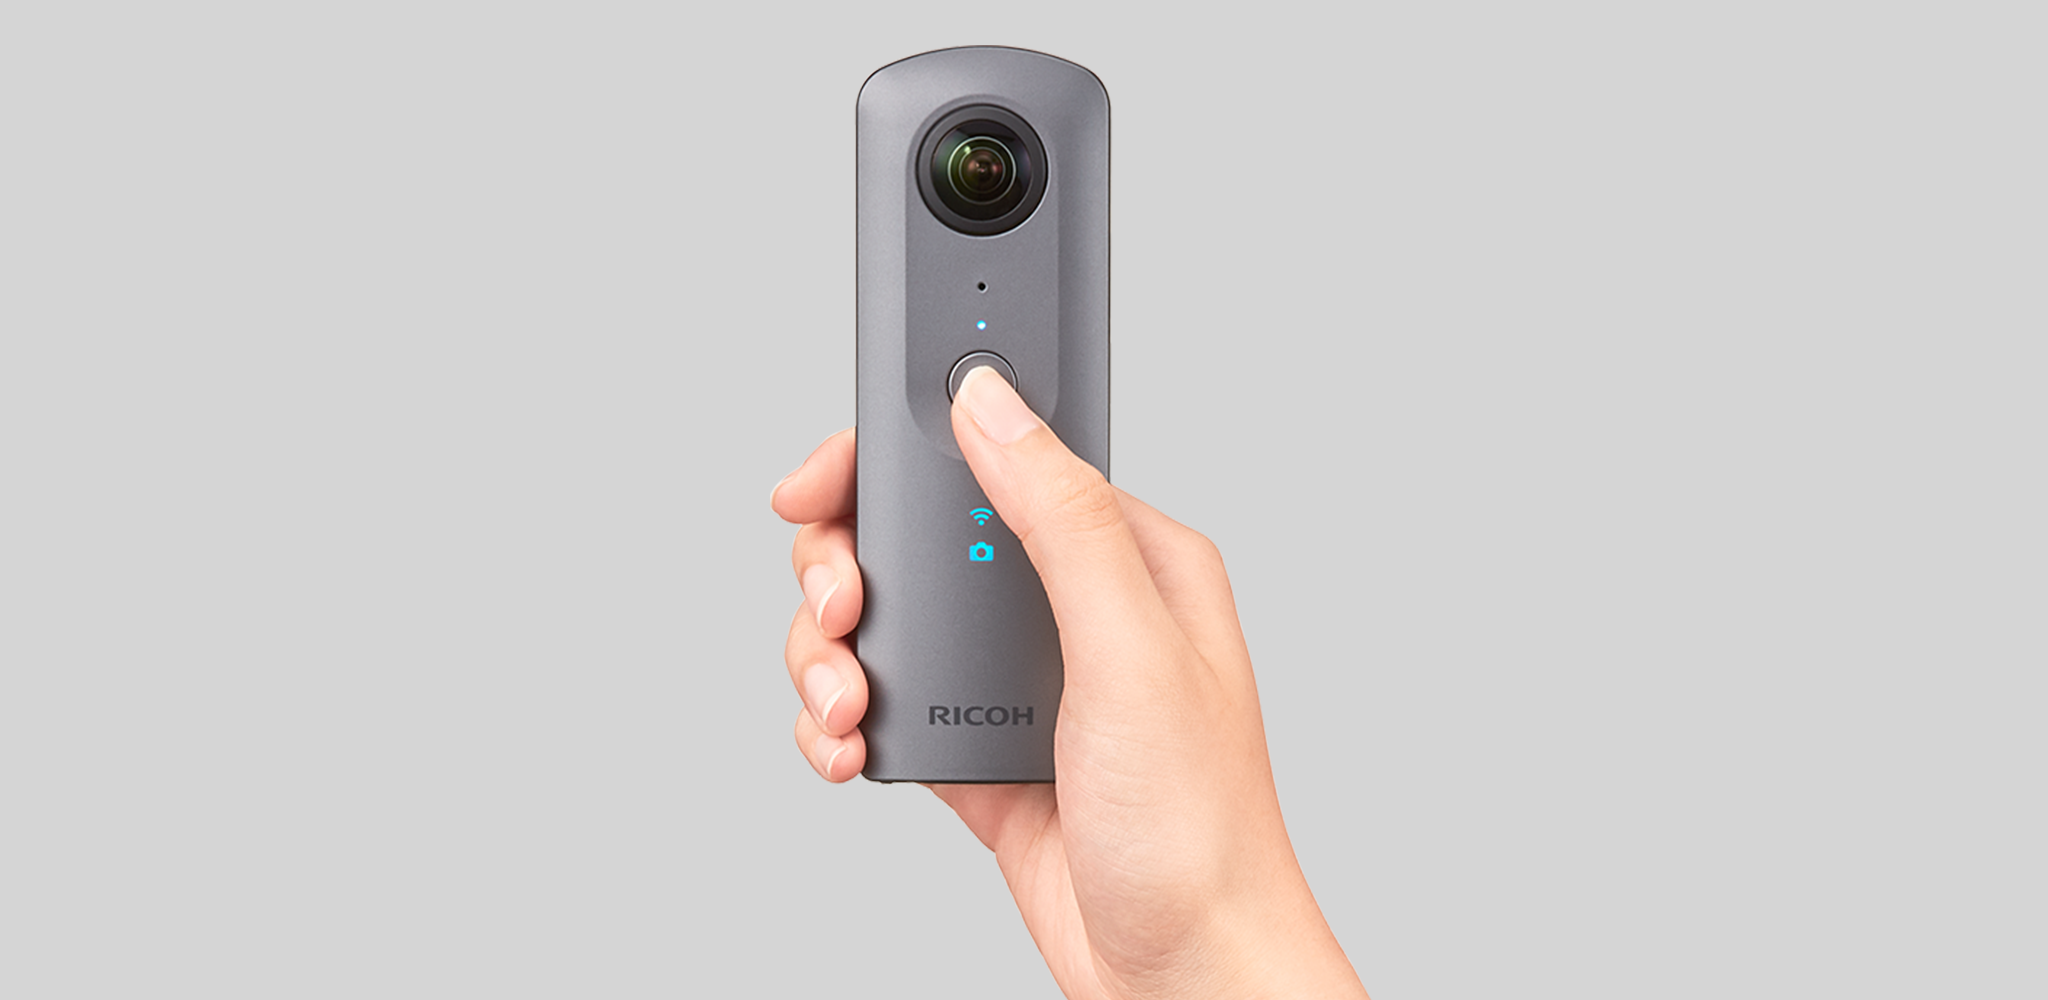
\includegraphics[scale=0.2]{fig/thetaV.png}
  \caption{全天球パノラマ画像}\label{fig:2}
\end{figure}
\begin{figure}[tb]
  \centering
  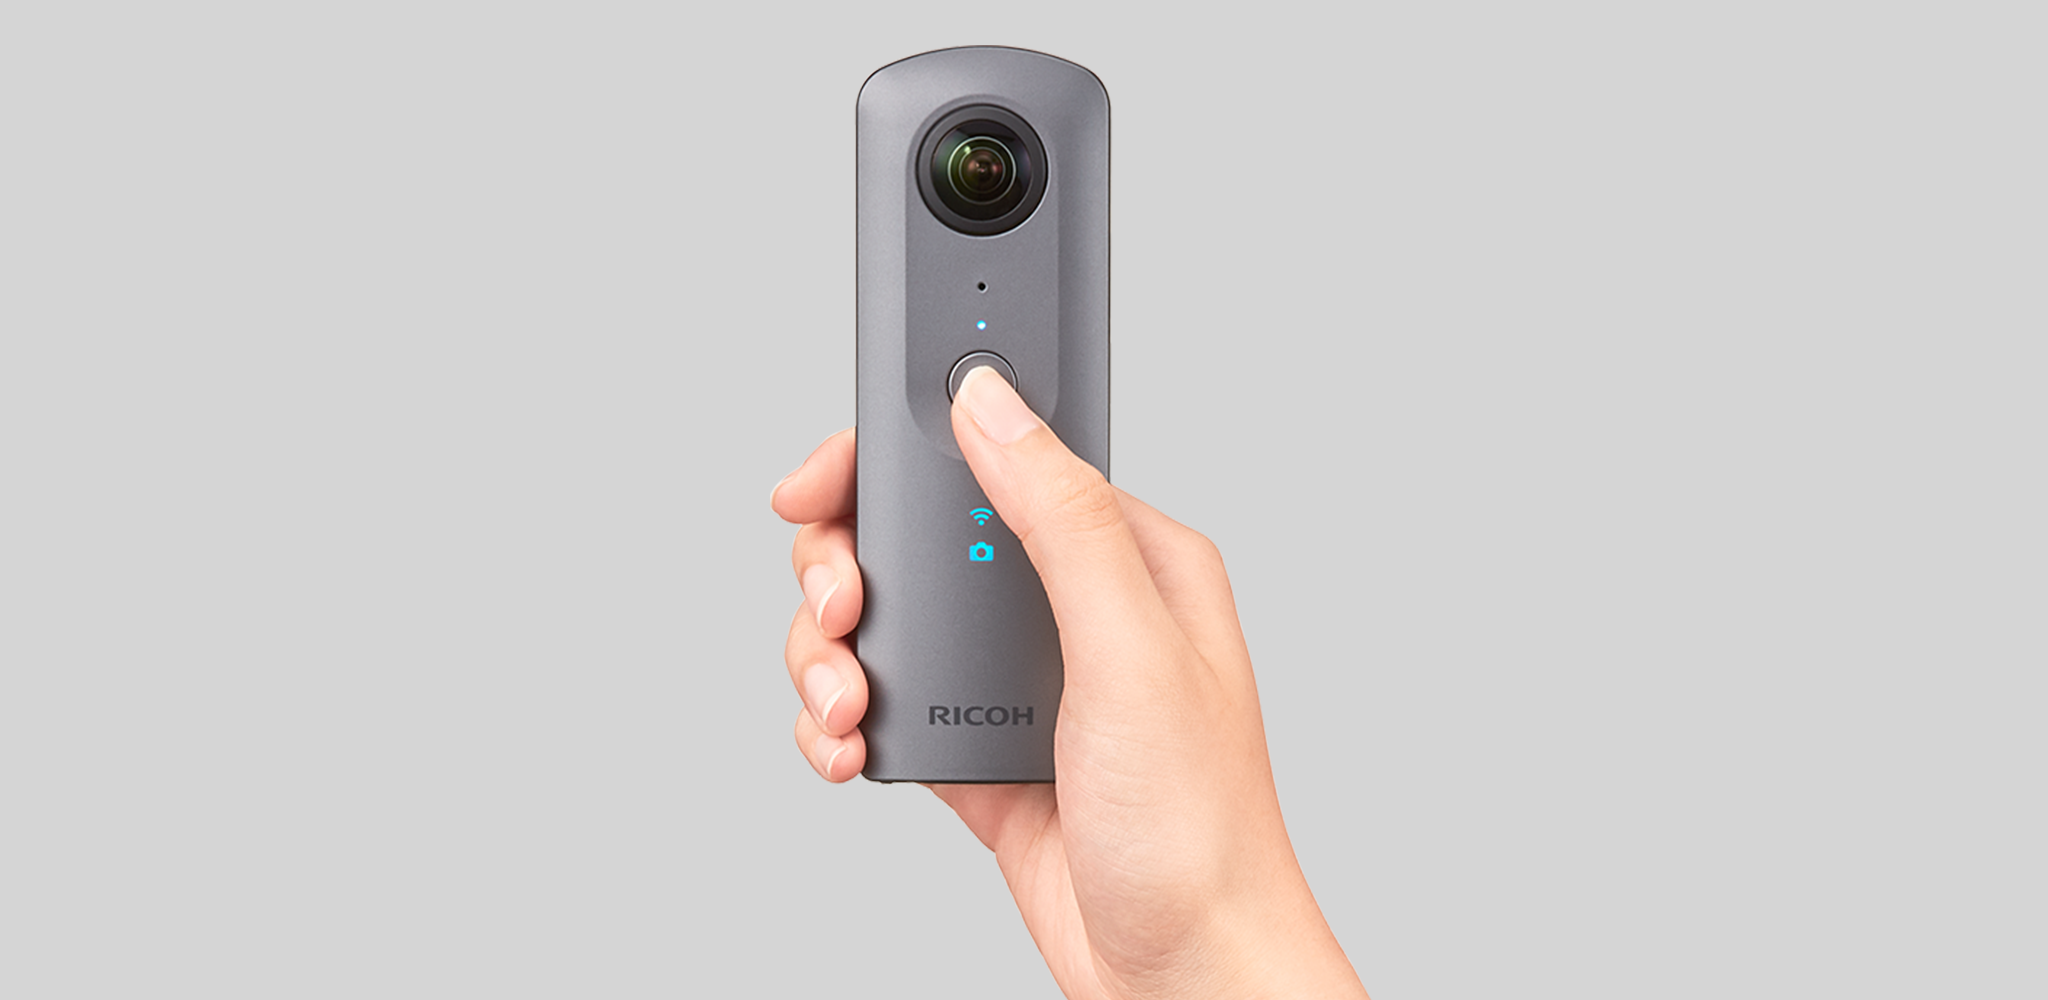
\includegraphics[scale=0.2]{fig/thetaV.png}
  \caption{theta V}\label{fig:3}\cite{4}
\end{figure}

全天周カメラの使用により、カメラの視野の問題は解決される。
実際に、Anthonyら\cite{5}は、全天球の視野の広さによって、リモートユーザーが
ローカルユーザーの環境をより早く理解できると結論付けている。
だが、Johnsonら\cite{6}によって、パノラマ視野によって映像の複雑さが増し、
より大きな認知負荷を必要としたことも示されている。

認知負荷を削減するため、パノラマ映像を3次元に表示する、球体プロジェクターを
用いた方法が挙げられる。球体プロジェクターの利用としては、LiらのOmniEyeBall
\section{本論文の構成}本論文の構成は以下のようになっている.

第2章では,本研究の関連研究として,
全天球カメラとそれに関する研究,球状ディスプレイ
に関する研究,及びビデオ会議に関する研究を紹介する.
第3章では,本論文で提案するビデオ会議システムに
ついての詳細を述べ,第4章ではその実装を具体的に
記述する.
第5章では,本研究で行った実験について仔細を述べ,
実験結果,及びそれに対する考察を記す.
第6章では第5章での実験結果に基づいて,実験で
用いたアプリケーションの問題点を述べる.加えて,作成した
3つのアプリケーションについて,詳細と具体的な実装を
述べたのち,本研究での限界と,今後の研究課題について述べる.
第7章では,それまでに記述した内容を踏まえ,総括と結論を
述べる.

\chapter{関連研究}
%\section{本章の概要}
\section{360度カメラに関する研究}\begin{itemize}
  \item RICOH THETA V(https://theta360.com/ja/about/theta/v.html)
  \item insta 360(https://www.insta360.com/jp/product/insta360-onex2)
  \item Meeting OWL(http://meetingowl.jp/?i=nav)
  \item Collaboration in 360° Videochat: Challenges and Opportunities(https://dl.acm.org/doi/10.1145/3064663.3064707)
\end{itemize}
\section{全天周球状ディスプレイに関する研究}\begin{comment}
\begin{itemize}
  \item Glomal350(https://www.aisan.co.jp/products/glomal350.html)
  \item WORLDEYE(https://www.gakkensf.co.jp/worldeye/sp/)
  \item OmniEyeball: An Interactive I/O Device For 360-Degree Video Communication(https://dl.acm.org/doi/10.1145/3279778.3279926)
  \item Qoom: An Interactive Omnidirectional Ball Display(https://dl.acm.org/doi/10.1145/3126594.3126607)
  \item Comparing flat and spherical displays in a trust scenario in avatar-mediated interaction(https://dl.acm.org/doi/10.1145/2556288.2557276)
\end{itemize}
\end{comment}

\subsubsection*{球体ディスプレイ}

球体ディスプレイの例として,渋谷工学のGlomal350\cite{15}や学研の
WORLDEYE\cite{22},WataruらのiSphere\cite{23}がある.
球体ディスプレイには
\begin{itemize}
  \item リアプロジェクション型
  \item フロントプロジェクション型
  \item 発光型
\end{itemize}

の3種類が存在する.リアプロジェクション型は,ディスプレイの裏側から
映像投影を行う.フロントプロジェクション型は,ディスプレイの外側から
映像投影を行う.一方で,発光型は,球の構成自体を,有機EL等の
発光装置で行い,球それ自体が発光する.Glomal550やWORLDEYEは,リアプロジェクション型
の球体ディスプレイである.
一方でiSphereは,ドローンに発光LEDを取り付けて回転させて球状
映像を表示する,発光型の球体ディスプレイである.(表\ref{isphere})
\begin{figure}[tp]
  \centering
  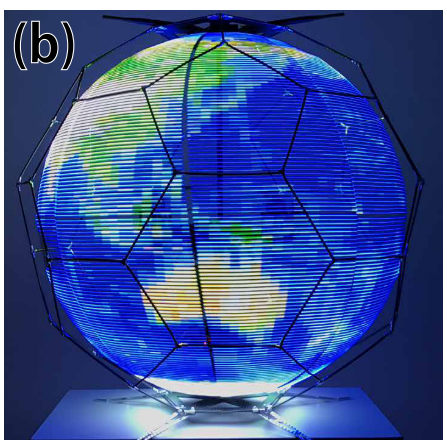
\includegraphics[scale=1.0]{fig/isphere.png}
  \caption{iSphere\cite{23}}\label{isphere}
\end{figure}

リアプロジェクション型の球体ディスプレイは,球内部に
魚眼レンズを取り付けており,また殆どの魚眼レンズは
等距離射影方式を採用している.等距離射影方式は,
レンズへの光の入射角を$\theta$,スクリーンへの
光の到達点と光軸との距離を$R$,焦点距離を$f$とすると
以下の式が成り立つ射影方式である.(図\ref{pro})

\begin{eqnarray}
  R = f\theta \nonumber \\
\end{eqnarray}

\begin{figure}[tp]
  \centering
  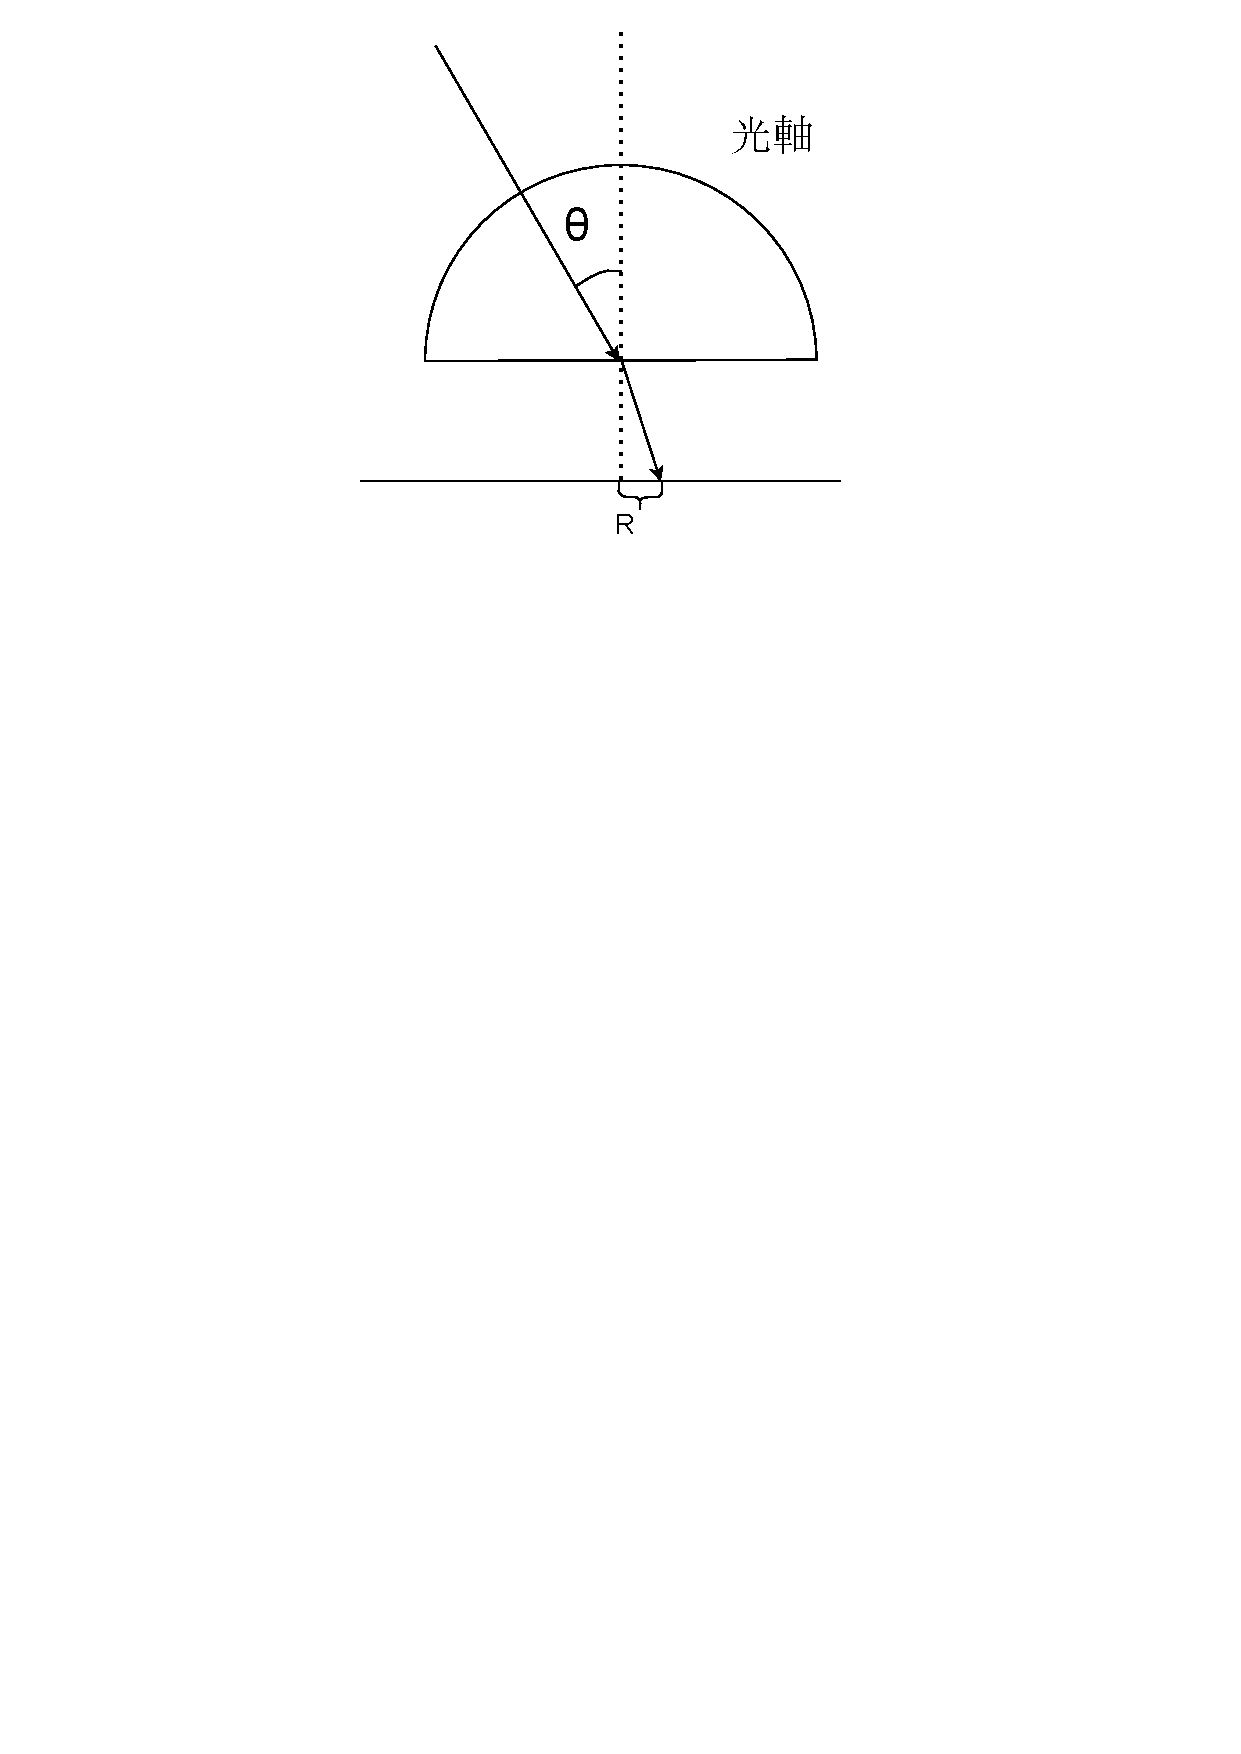
\includegraphics[scale=0.7]{fig/projection2.pdf}
  \caption{等距離射影方式の模式図}\label{pro}
\end{figure}

すなわち,投影元の画像中心からの距離に比例して,投影先の球体上での
天頂からの角度が比例する.よって,魚眼レンズを使用したリアプロジェクション型の
球体ディスプレイを利用する際には,投影元の映像を正距方位図法(図\ref{teiso3})へと
変換しておく必要がある.

\begin{figure}[tp]
  \centering
  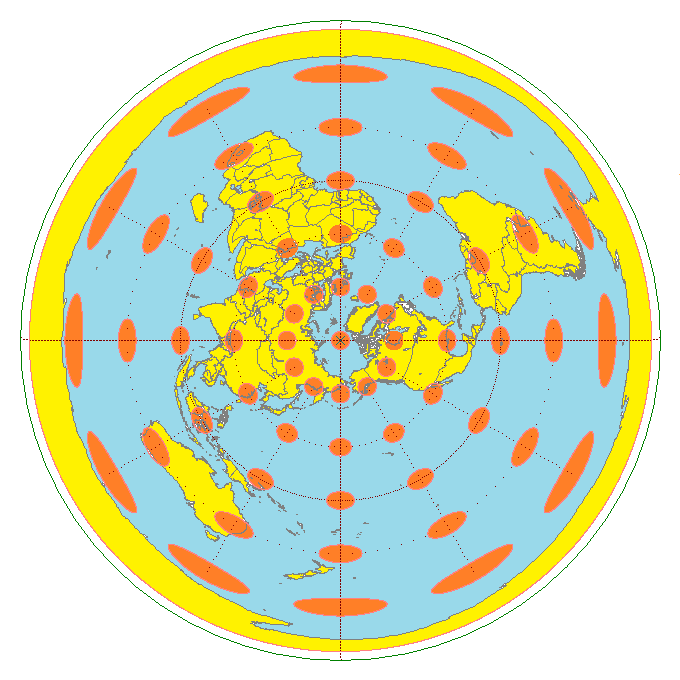
\includegraphics[scale=0.8]{fig/teiso3.png}
  \caption{正距方位図法\cite{20}}\label{teiso3}
\end{figure}

\subsubsection*{球体ディスプレイの応用}
球体ディスプレイと全天球ビデオカメラを用いた例として,Liらの
OmniEyeBall\cite{18}\cite{24}がある.OmniEyeBallは,
glomal350を映像プロジェクターとして用いて,球体ディスプレイの
天頂部に広角の魚眼レンズを取り付けたデバイスである.(図\ref{proto})
\begin{figure}[tp]
  \centering
  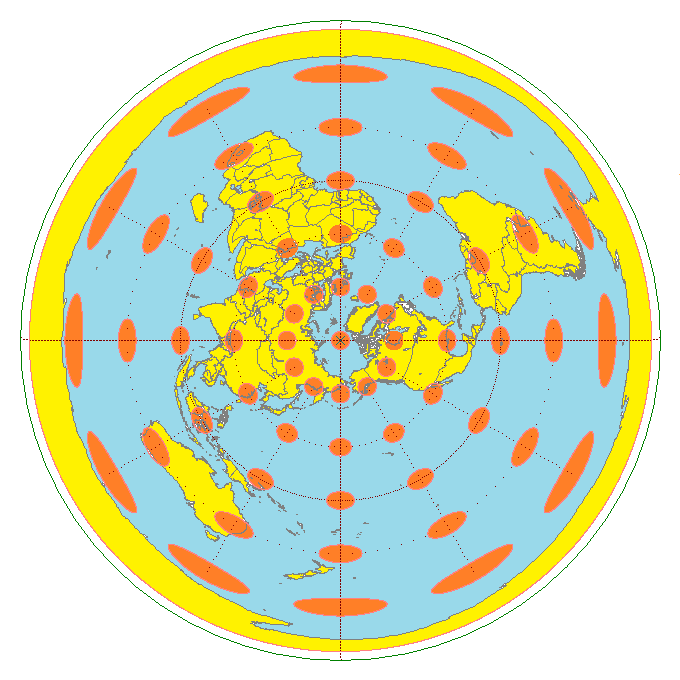
\includegraphics[scale=0.6]{fig/teiso3.png}
  \caption{OmniEyeBallの構成の概要\cite{24}}\label{proto}
\end{figure}

2台のOmniEyeBallを用いて,魚眼レンズの映像のストリーミングを行うことで,
OmniEyeBallを複数人で囲う形のビデオ会議が可能である.
OmniEyeBallをもちいたビデオ会議実験では,平面ディスプレイでの表示では
歪みが強い,球体ディスプレイでの表示は距離や方向感覚がつかみやすい
といった内容が報告されている.また球体ディスプレイを用いた方が
特定の個人とのコミュニケーションがしやすくなったことが示されており,
一方で平面ディスプレイ時には多対多のコミュニケーションが多く行われたことが
示された.

Miyafujiら\cite{25}は,複数のプロジェクターとモーションキャプチャーを
利用して,動くボールに対してプロジェクションマッピングを行い,ボールを
フロントプロジェクション型の球体ディスプレイとして利用するQoomを提案した.
Qoomでは,ボールに対して触れる,回す,地面に投げる,人に投げるといった,人が
ボールに対して行う自然な動作に対して,それぞれに対応した挙動をするように設計されている.

\begin{figure}[tp]
  \centering
  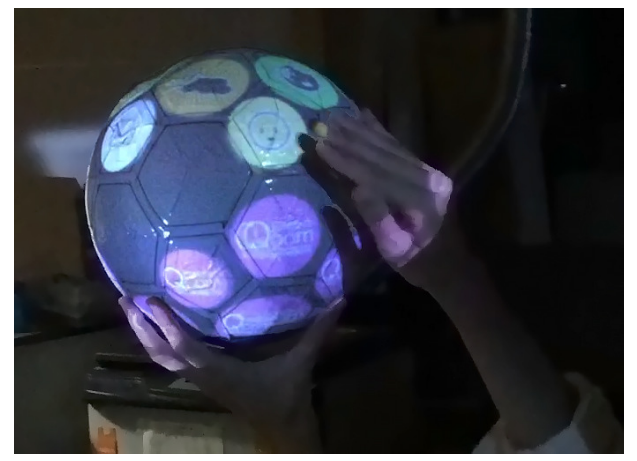
\includegraphics[scale=0.9]{fig/qoom.png}
  \caption{Qoom\cite{25}}
\end{figure}

\begin{figure}[tp]
  \centering
  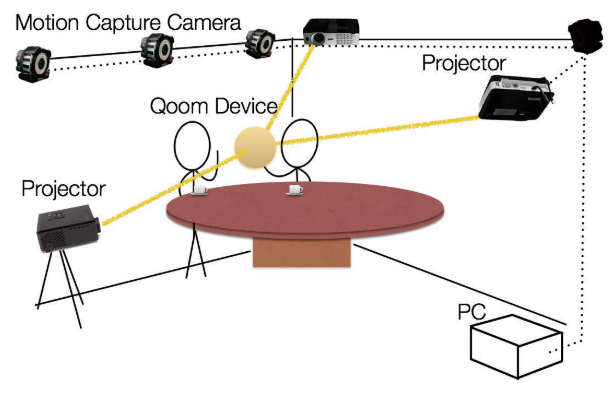
\includegraphics[scale=1.0]{fig/qoomsys.png}
  \caption{Qoomの構成の概要\cite{25}}
\end{figure}

Panら\cite{26}は,平面ディスプレイと球体ディスプレイで
アバターの表示に関する比較の研究を行った.実験の内容は,
30個の難解な質問に対し,声と容姿は同一で正答率の異なるアバターを,
平面ディスプレイと球体ディスプレイのそれぞれに表示し,どちらか片方のみから
答えを聞くというものであった.(図\ref{avaterexp})結果,被検者は球体ディスプレイの
アバターを多く選択する結果が得られている.特に,ディスプレイの距離
の差が広いほど,球体ディスプレイを選択する傾向にあったことが示された.
被検者のアンケートでは,アバターの動きや声の演者は同一であるのにもかかわらず
\begin{itemize}
  \item エマの目はサポート感があるが、ケイティの声の方が説得力がある
  \item ケイティはいつも答えに自信があるように見えるが、エマは自分の知っていることを話しているように見える
\end{itemize}
などの意見が見られていた.

\begin{figure}[tp]
  \centering
  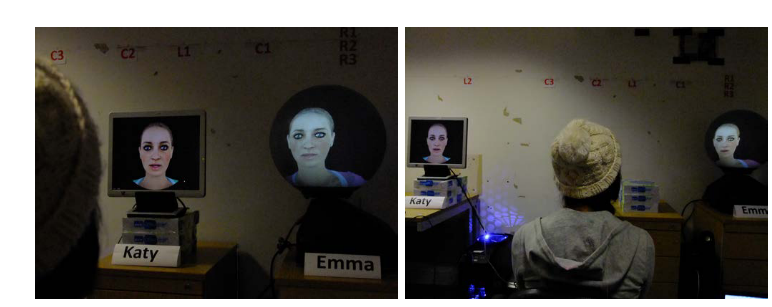
\includegraphics[scale=0.6]{fig/avaterexp.png}
  \caption{Panらの実験の様子\cite{26}}\label{avaterexp}
\end{figure}



\section{ビデオ会議に関する研究}\begin{comment}
\begin{itemize}
  \item Room2Room: Enabling Life-Size Telepresence in a Projected Augmented Reality Environment(https://dl.acm.org/doi/pdf/10.1145/2818048.2819965)
  \item Improving visibility of remote gestures in distributed tabletop collaboration(https://dl.acm.org/doi/10.1145/1958824.1958839)
  \item Putting things in focus: establishing co-orientation through video in context(https://dl.acm.org/doi/10.1145/2470654.2466174)
  \item A gaze-preserving group video conference system using screen-embedded cameras(https://dl.acm.org/doi/10.1145/3139131.3141775)
  \item Towards Enabling Eye Contact and Perspective Control in Video Conference (https://dl.acm.org/doi/10.1145/3379350.3416197)
\end{itemize}
\end{comment}
Pejsaら\cite{27}は,投影型の拡張現実環境を用いて,対面時の
ような1対1の遠隔会議が出来るシステムを考案した.Kinnectによって
参加者の動きや体勢を認識して,3Dモデルを自動生成して,相手の
正面へと表示することで,疑似的な対面環境を作り出した.
実験の結果,従来のビデオ会議を用いたコミュニケーションよりも
通信相手の存在感や,コミュニケーションの効率といった観点で
優れていることが示された.一方で,解像度の低さなどの問題から
,ジェスチャーを用いたコミュニケーションの頻度が低下したことや,
1対1のケースに用途が限られている等の問題点が指摘されている.
\begin{figure}[tp]
  \centering
  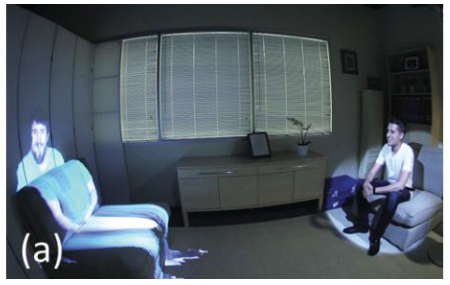
\includegraphics[scale=1.2]{fig/2room2.png}
  \caption{Room2Roomによる通信の様子\cite{27}}
\end{figure}

Yamashitaら\cite{28}は,卓上での作業における遠隔ビデオ会議
において,ジェスチャーの情報が失われることを指摘し,卓上
において遠隔参加者のジャスチャーが視認できるシステムt-Roomを
提案した.卓上ディスプレイに遠隔地参加者のジェスチャーを表示する
際には,物体にさえぎられるなどの問題がある.そこで,リモートラグと呼ばれる
,遠隔地参加者の遅延した映像をリアルタイム映像と同時に表示することで,
ジェスチャーの理解の正誤判断を行えるようにした.
通常表示条件とリモートラグ表示条件での比較実験の結果,ユーザーは
見落としたジェスチャーの情報などを後から再認識することに成功し,ジェスチャー
を見落とすことによる不要な会話が減少したことが示されている.また,作業参加者の
体感作業負荷を減少させたことも示されている.

\begin{figure}[tp]
  \centering
  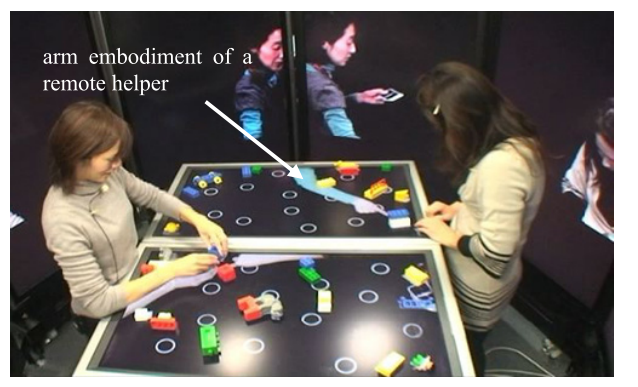
\includegraphics[scale=0.7]{fig/tRoom.png}
  \caption{t-Roomを使用する様子\cite{27}}
\end{figure}

\begin{figure}[tp]
  \centering
  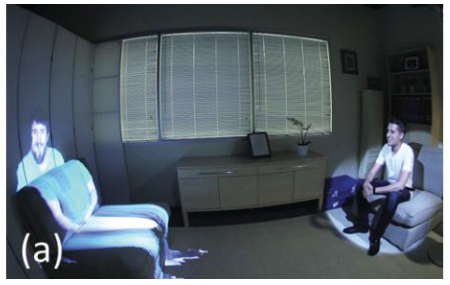
\includegraphics[scale=1.0]{fig/2room2.png}
  \caption{t-Roomの構成\cite{27}}
\end{figure}

Kobayashiら\cite{29}は,Kinnectと,複数のカメラから視線方向の推定を行い,
リアルタイムで,対面時の会話と同じ景色を再現する映像表示方法を提案した.(図\ref{Kobayashi})
Kobayashiらは,2対2でのコミュニケーションを行うケースを想定しており,以下の
場合について表示方法の切り替えを行った.
\begin{itemize}
  \item 一方の側の人物が他方の側のユーザに見られていない場合は,デフォルトの視点位置を使用する.
  \item  一方の面の人物が他方のユーザからのみ見られている場合は,そのユーザの視点位置を使用する.
  \item  一方の面の人物が他方の面の複数のユーザから見られている場合は,お互いを見ているペアを使用する.
\end{itemize}

\begin{figure}[tp]
  \centering
  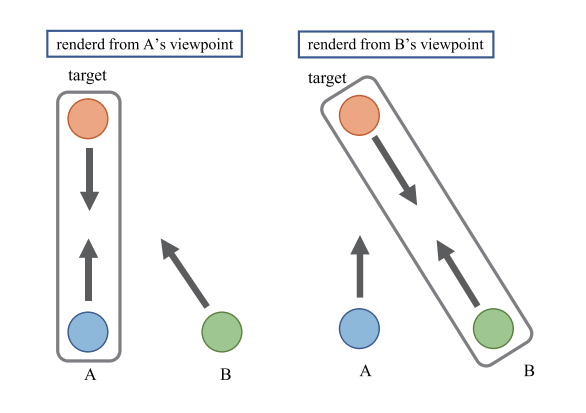
\includegraphics[scale=0.8]{fig/gaze.png}
  \caption{Kobayashiらの提案\cite{29}}\label{Kobayashi}
\end{figure}

\begin{figure}[tp]
  \centering
  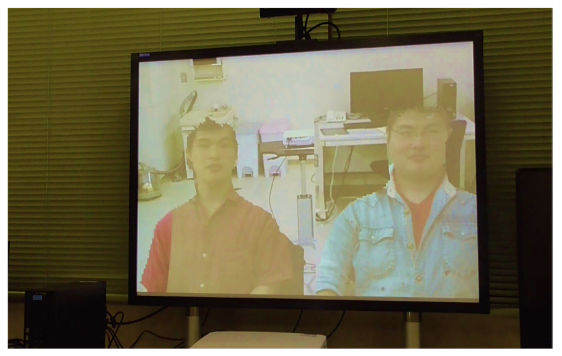
\includegraphics[scale=0.8]{fig/kobayashi2.png}
  \caption{Kobayashiらの提案システムのデモンストレーション\cite{29}}
\end{figure}




\section{まとめ}2-1節では,全天球カメラの概要と,全天球カメラ自体の問題点について指摘した.
全天球カメラは魚眼レンズを主に使用しており,パノラマ
画像の生成時には歪みがどうしても発生してしまう.
また,全天球カメラの視野の広さは,メリットが大きいものの,従来のカメラ映像には
存在しなかった新たな問題を引き起こした.

2-2節では,全天球ディスプレイと,全天球ディスプレイを使用した研究について
紹介した.全天球ディスプレイを用いたビデオ会議システムがいくつか提案されており,
立体感という観点から,ユーザーから高い評価を受けており,これが本研究でも
全天球ディスプレイを使用する動機になっている.

2-3節では,ビデオ会議に関する研究をいくつか紹介した.
ビデオ会議では対面でのコミュニケーションで得られるはずの
情報が失われ,その情報を再現するための研究が行われている.
そのような情報は,再現した結果有効に働いており,ビデオ会議における
臨場感の向上には必要であるといえる.

以上の流れをふまえ,3章で本研究における1対多人数の
ビデオ会議システムの提案を行う.

\chapter{球体ディスプレイを用いた視線共有システムの提案}
%\section{本章の概要}
\section{従来型ビデオ会議アプリケーションの問題点}%・全天球映像は視野が広い

%・ビデオ会議では視線情報が失われる

%・誰がどこを見ているのかという情報が必要

%・(上記の根拠として,2で関連研究を提示する)

ビデオ会議では,視野の狭さにより,参加者同士の状況が分かりづらいという欠点がある.
そのため,コミュニケーションが円滑に行われない場合がある.全天球ビデオカメラを使用することで
視野の狭さの問題が解決するが,一方で映像が複雑になり,その影響でやはり快適なコミュニケーションが
行われない可能性がある.

一方で,2-2節で述べたOmniEyeBallに代表される,全天周ディスプレイを用いたビデオ会議が考えられる.
全天周ディスプレイでは,全天球映像が球を用いた立体的かつ自然な形で表現され,全天球映像を視認
しやすくなる.

しかし,上記の方法でなお,視線情報の問題が存在する.これは,カメラ画像から発話者の視線が取得困難であったり,
発話者の視線が考慮されたディスプレイ上での表示が行われていない,といった
コミュニケーションにおいて重要であるにもかかわらず従来のビデオ会議では未だに未解決の問題である.
以下では,PCの使用者1人とOmniEyeBallの使用者複数人の非対称な通話状況において,PC使用者の視線情報を伝える方法を提案する.




\section{提案する視線共有システム}%・(PC側では)クリックした人間の映像を正面に持ってくることで,正面を見ていれば見たい人を物理的にも見ているという状態を作る

%・(OEB側では)PC側が見ている特定の個人の方向に,PC使用者の顔を映す

%・残りの人間には,PC側と,見ている人間の顔を小さいウインドウに移し,視線情報と通信相手の顔を伝える

%・特定の1人を見ていない状況を区別するため,そのような状況下では全員にPC使用者の顔を小さいウインドウに移す

PC側で提案するシステムを以下に述べる.平面ディスプレイ上に
OmniEyeBallに取り付けた全天球ビデオカメラのパノラマ映像を表示する.
映像上で,参加者の顔をクリックすることで,その参加者が正面に来るように
パノラマ映像を平行移動させる.そのようにして,常に正面を見ていれば
見たい人を見ているという状態を作り出す.

%(ここに,画像をスライドさせる図を乗せる)
\begin{figure}[tp]
  \centering
  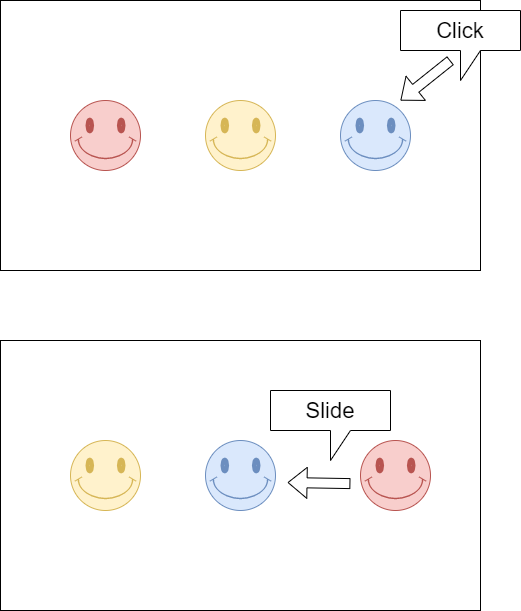
\includegraphics[scale=0.6]{fig/PCsideSlide.png}
  \caption{全天周パノラマ画像のスライド}
\end{figure}

以降は,OmniEyeBall側で提案するシステムを述べる.
PC側で使用する全天周ビデオカメラの映像を
球体ディスプレイ上に表示する.PC側のクリック操作に合わせ
クリックされた人物の方向に顔が向くように映像を回転させる.
こうすることで,PC側で見ている人間とみられた人間が向き合う状態を作る.

\begin{figure}[tp]
  \centering
  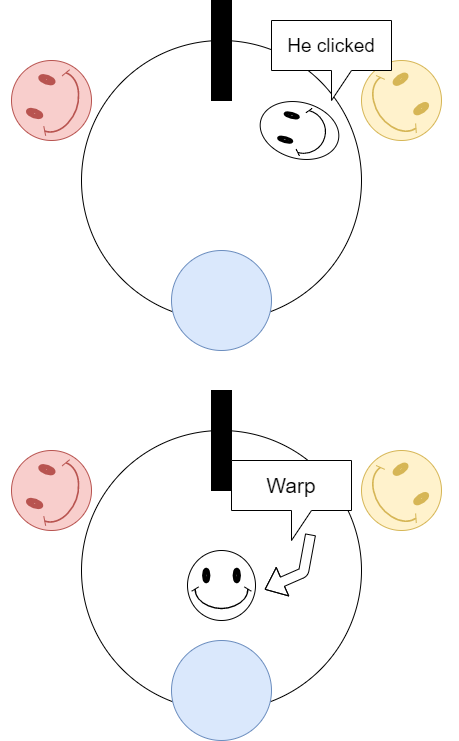
\includegraphics[scale=0.6]{fig/OEBsideSlideimg.png}
  \caption{クリックイベント発生時の全天球ディスプレイ上の表示}
\end{figure}

この時,例えば3人が120度の間隔でOmniEyeBallの周りに座っている状況を考えると,
顔を向けられていない2人は,ほとんどPC側の参加者の顔を視認できない.
このような場合,この2人には画面上部に小さなウインドウを表示し,そこに
PC側参加者の顔部分を表示する.顔部分を表示すると,その顔は大抵正面方向を向いており
,自身が見られていると錯覚する恐れがある.それを防ぐため,PC参加者の顔ウインドウ
の隣には,見られている参加者の顔ウインドウを表示させる.

また,このままではPC側の使用者が,特定の個人を見ていない場合
(例えば,全員に対して語りかける場合)を区別できない.このため,
特定の個人を見ていない場合は,全員に対して画面上部に
PC参加者のみの顔ウインドウを表示させる.クリックした人物の方向を向く
仕様では,常に前回のクリックの結果が残り,いずれかの人物の顔方向に
PC参加者の顔が向くことになる.この方向に対して,あえて顔ウインドウ
を顔映像に被せることによって,大きく表示される方の顔映像の視認性を下げ,
自身が見られているという錯覚を防ぐことが狙いである.

\begin{figure}[tp]
  \centering
  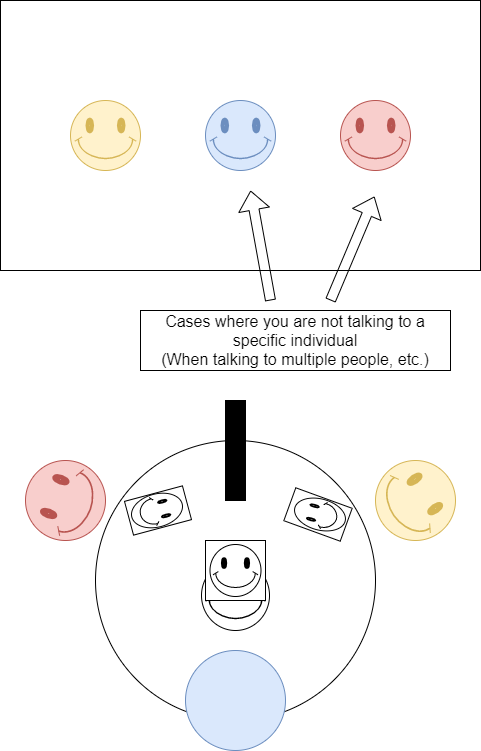
\includegraphics[scale=0.6]{fig/SPcase.png}
  \caption{特定の個人を見ていない場合の表示}
\end{figure}
\section{技術的課題}ハードウェア部分の実装に関しては,全天球ビデオカメラ2つ,PC2台,及び
OmniEyeBall1台を用意すればよい.

一方,ソフトウェア部分の実装に関しては,いくつか準備の必要がある
要素が存在する.

まず,ビデオストリーミングの方法について考える必要がある.
UDP等を用いて映像情報の送受信を行う必要がある.しかし,フレーム落ちの
問題など,現在使用されているビデオ会議アプリケーションのような堅牢で
高速な通信を実現するためには,高度な技術と時間を要する.
そこで,映像送受信については,すでに利用されているビデオ会議アプリケーション
を用いることにした.

しかし,ただ映像を送受信していては,PC側の操作に合わせて映像を回転させる
といった処理が出来ない.PC側では全天球ビデオカメラの映像を加工した後に
送信を行う必要がある.あるいは,PC側で表示するUIにおいて,OmniEyeBall側の
全天周パノラマ映像をそのまま表示させるのではなく,やはりクリックした人物の
顔を正面に移動させるなどの必要がある.
ここで,加工した映像をキャプチャしてビデオ会議アプリケーションに
認識させる方法と,一方で,送信されてきた映像をキャプチャーして,
以下で説明する画像加工ライブラリで扱えるようにする方法を考えなければならない.

この両方を解決するために,今回は仮想ビデオカメラを用いる.
仮想ビデオカメラとは,OBS-virtual-cam\cite{7}やUnityCapture\cite{8}
等のような,特定のアプリケーションの映像をリアルタイムでキャプチャし,
その映像をあたかも接続したビデオカメラの映像のように扱えるものである.
これを用いることで,ビデオ会議アプリケーションや画像加工ライブラリ
が,加工済みの映像や送信されてきた映像をビデオカメラの映像として認識し,
ストリーミングや加工が出来るようになる.

(以下に,映像送受信+加工のフローの図を乗せる)

次に,映像の加工方法について述べる.映像の加工はpythonなどで利用可能な
画像加工ライブラリを用いた.同時にPC画面に表示するUIもpythonのライブラリで作成した.

\chapter{OmniEyeBall対PC間通信の実装}
%\section{本章の概要}
%\section{本研究の内容と提案手法}・ビデオストリーミングの実装の手間を省くため,画像送受信にはZoomとOBS studioを用いた

・見ている人をクリックすると,OEB側でその方向を向くことで,視線情報を伝えた

・顔が見えなくなる問題は,すべての人間に小窓を表示することで解決した

・また,小窓で正面を向いており,見られていると錯覚するのを防ぐため,隣には現在見られている相手を表示した

・特定の個人に話しかけていない状態を区別するため,そのようなときは全員にPC使用者のみの小窓を表示した

・PC側では,常に正面を向いていれば見たい人を正面に見据えられるように,クリックした人間の顔を正面に持ってくる処理を施した

・(以下4-2-1から5では,システムが動く様子を表した図や画像を用意する)

%\section{本研究の実装}
%  \subsection{360度カメラ}・RICHO THETA V

・RICHO THETA S
%  \subsection{OmniEyeBall}・(OmniEyeBall)4K画質球体ディスプレイを使用

・glomal360

%  \subsection{オンラインビデオストリーミング}・送受信にはzoomを用いた

・加工後や,加工前の映像を仮想カメラ映像としてキャプチャするため,OBS virtual camを用いた

・(OEBにうつす映像)THETA Sで撮影した映像をOpenCVで加工->OBSでキャプチャ->zoom

・(PCに移す映像)THETA Vで撮影した映像をZoomで送信->OBSでキャプチャ->OpenCV + TKinterで加工
%  \subsection{OpenCVを用いた360度パノラマ画像の処理}・OBS studioでキャプチャ

・OpenCV4で加工

・OEB用の画像は,パノラマ画像を極座標変換して作成

・PC用の画像は,OpenCVで不要な領域を削除

%  \subsection{GUIアプリケーション}・TKinterを使用

・クリックイベントを追加,クリックした場所で誰を見ているか判断し,真ん中に持ってくる

・上のクリックイベントと同時に,OpenCVで小窓を作成
  \section{ハードウェア実装}%・RICHO THETA V

%・RICHO THETA S

%・(OmniEyeBall)4K画質球体ディスプレイを使用

%・glomal360

\subsection*{全天周ビデオカメラ}
全天周ビデオカメラとして,PC側ではRICOH THETA S,
OmniEyeBall側ではRICOH THETA Vを用いた.
\begin{table}[tp]
  \begin{center}
    \begin{tabular}{|c|c|}
      \hline
      記録媒体                                                             & 内蔵メモリー:約8GB                                                                                                                                                    \\ \hline
      記録可能枚数, 時間                                                       & \begin{tabular}[c]{@{}l@{}}静止画:(L)約1600 枚, (M)9000 枚\\ 動画(1 回の記録時間)\\ :最大25 分もしくはファイルサイズの上限4GB\\ 動画(合計記録時間)\\ :(L) 約65 分, (M) 約175 分\end{tabular}              \\ \hline
      圧縮方式                                                             & \begin{tabular}[c]{@{}l@{}}静止画:JPEG(Exif Ver2.3) DCF2.0 準拠\\ 動画:MP4(映像:MPEG-4 AVC/H.264, 音声:AAC)\\ ライブストリーミング\\ :(USB)MotionJPEG, MPEG-4 AVC/H264\end{tabular} \\ \hline
      静止画解像度                                                           & \begin{tabular}[c]{@{}l@{}}L:5376 × 2688\\ M:2048 × 1024\end{tabular}                                                                                          \\ \hline
      \begin{tabular}[c]{@{}l@{}}動画解像度/フレームレート/\\ ビットレート\end{tabular}  & \begin{tabular}[c]{@{}l@{}}L:1920 × 1080/30fps/16Mbps\\ M:1280 × 720/15fps/6Mbps\end{tabular}                                                                  \\ \hline
      \begin{tabular}[c]{@{}l@{}}ライブストリーミング解像度/\\ フレームレート\end{tabular} & \begin{tabular}[c]{@{}l@{}}L:1920 × 1080/30fps\\ M:1280 × 720/15fps\end{tabular}                                                                               \\ \hline
      \end{tabular}
  \caption{THETA Sの仕様} \cite{4}
  
  \begin{tabular}{|c|c|}
    \hline
    記録媒体                                                             & 内蔵メモリー:約19GB                                                                                                                                                                    \\ \hline
    記録可能枚数, 時間                                                       & \begin{tabular}[c]{@{}l@{}}静止画:約4800枚\\ 動画(1 回の記録時間)\\ :最大25 分\\ 動画(合計記録時間)\\ :130分(2K, H264)\end{tabular}                                                                      \\ \hline
    圧縮方式                                                             & \begin{tabular}[c]{@{}l@{}}静止画:JPEG(Exif Ver2.3)\\ 動画:MP4(映像:MPEG4 AVC/H.264,H.265 *7、\\ 音声:AAC-LC(モノラル)+Linear PCM(4ch空間音声))\\ ライブストリーミング:(映像:H.264、音声:AAC-LC(モノラル))\end{tabular} \\ \hline
    静止画解像度                                                           & 5376×2688                                                                                                                                                                       \\ \hline
    \begin{tabular}[c]{@{}l@{}}動画解像度/フレームレート/\\ ビットレート\end{tabular}  & \begin{tabular}[c]{@{}l@{}}4K,H264:3840×1920/29.97fps/56Mbps\\ 2K,H264:1920×960/29.97fps/16Mbps\end{tabular}                                                                    \\ \hline
    \begin{tabular}[c]{@{}l@{}}ライブストリーミング解像度/\\ フレームレート\end{tabular} & \begin{tabular}[c]{@{}l@{}}4K,H264:3840×1920/29.97fps/120Mbps\\ 2K,H264:1920×960/29.97fps/42Mbps\end{tabular}                                                                   \\ \hline
    \end{tabular}
    \caption{THETA Vの仕様} \cite{4}
  \end{center}
\end{table}

\subsection*{球体ディスプレイ}
全天球動画の出力装置としては
渋谷光学の球体プロジェクターであるGlomal350を使用する.
\begin{table}[tp]
  \begin{center}
    \begin{tabular}{|c|c|}
      \hline
      外形寸法    & \begin{tabular}[c]{@{}l@{}}幅450X奥行460X高さ600mm\\      球体サイズ:φ350mm\end{tabular} \\ \hline
      投影方式    & 1clip DLP方式                                                                    \\ \hline
      表示素子サイズ & XGA0.55型(アスペクト比4:3)                                                            \\ \hline
      画素数     & 786,432画素(1024X768)                                                            \\ \hline
      明るさ     & 2700lm                                                                         \\ \hline
      HDMI信号  & \begin{tabular}[c]{@{}l@{}}圧縮表示:\\      最大1920X1080(HD TV 1080p)\end{tabular}  \\ \hline
      \end{tabular}
  \caption{Glomal 350の仕様} \cite{15}
  \end{center}
  \end{table}
  \section{ソフトウェア実装}\subsection*{映像ストリーミング}
全天球映像の送受信にはZoom Video Communicationsの
Zoom\cite{1}を使用した.

\begin{table}[tbp]
  \begin{center}
  \begin{tabular}{cc}
  最大解像度 & 1280x720 \\
  最大fps & 30      
  \end{tabular}
  \caption{Zoomの仕様}
  \end{center}
  \end{table}

\subsection*{仮想カメラ}
映像のキャプチャ手段としてOBS Studio\cite{9}を用いている.
OBS Studioは起動中のアプリケーションや画面全体,接続されたカメラ
の映像をキャプチャー・合成して作成した映像をYoutube等の動画配信サイトへ
ストリーミングできるアプリケーションである.
以下の図のタイマーのキャプチャのように,キャプチャしてきたアプリの
映像にエフェクトを加えることも可能である.(映像では青色のクロマキーフィルタを
加え,背景を透明にしている)

\begin{figure}[tbp]
  \centering
  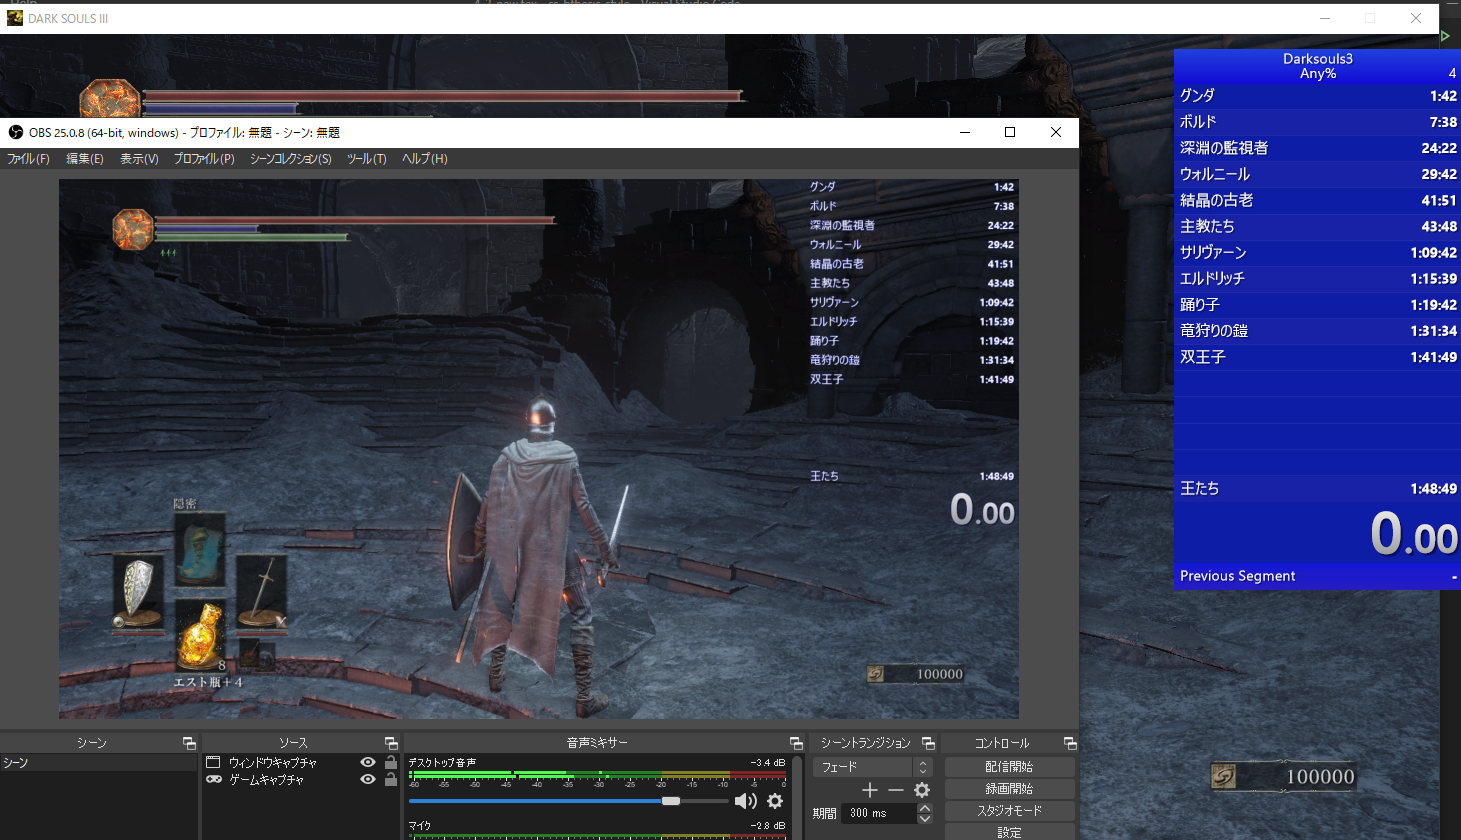
\includegraphics[scale=0.4]{fig/OBSstudio.png}
  \caption{OBSStudioで画面をキャプチャする様子}
\end{figure}

仮想カメラとしては,OBS-virtual-cam\cite{7}を
用いた.この仮想カメラの仕様は以下のようになっている.
 

\begin{table}[tbp]
  \begin{center}
  \begin{tabular}{cc}
  最大解像度 & 1280x720 \\
  最大fps & 60      
  \end{tabular}
  \caption{OBS-virtual-camの仕様}
  \end{center}
  \end{table}

OBS-virtual-cameraはOBS Stuioの機能であり,これを用いればOBS Studio
でキャプチャ中の映像を,仮想カメラの映像として扱うことが出来るようになる.
仮想カメラは,他アプリケーションからPCに物理的に付属したカメラと同様に
認識され,ストリーミングや映像の加工などが容易になる.

\begin{figure}[tbp]
  \centering
  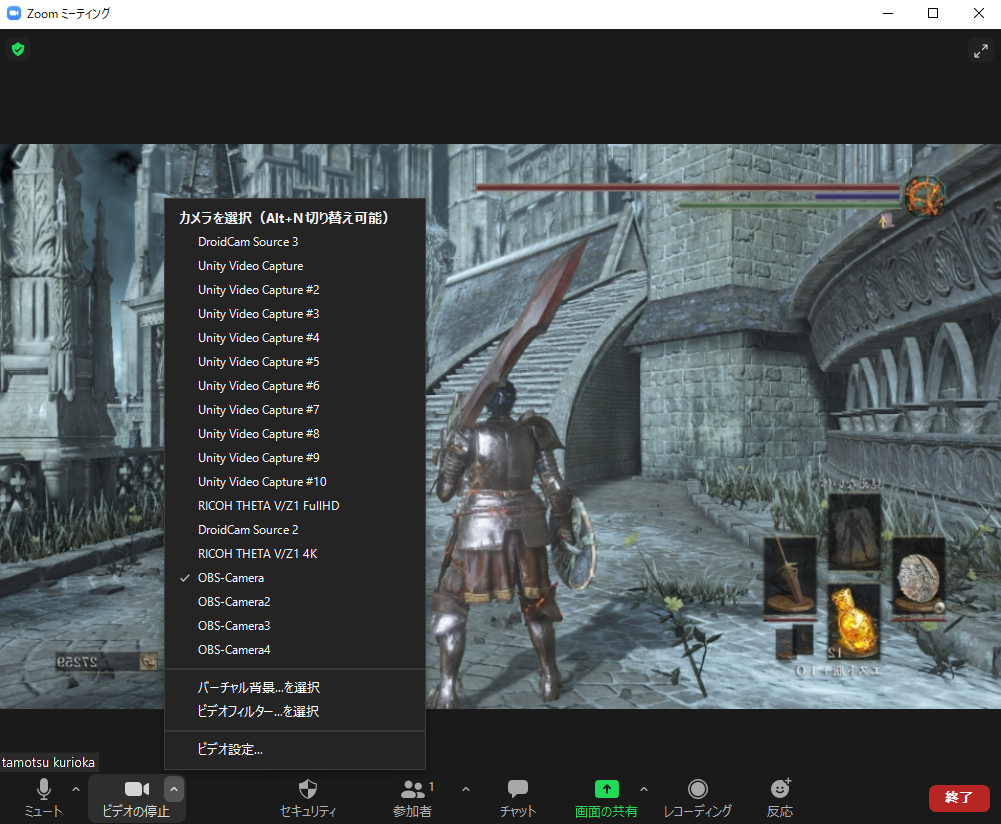
\includegraphics[scale=0.5]{fig/streaming.png}
  \caption{zoomでのOBS-virtual-camの映像ストリーミング}
\end{figure}

\subsection*{映像の加工}
映像の加工には,pythonのライブラリの1つであるOpenCVを用いた.
先述した通り,全天球ビデオカメラのパノラマ映像は正距円筒図法を用いて
出力されている.glomal350を用いる際にはさらに正距方位図法に変換
する必要がある.

\begin{figure}[tbp]
  \centering
  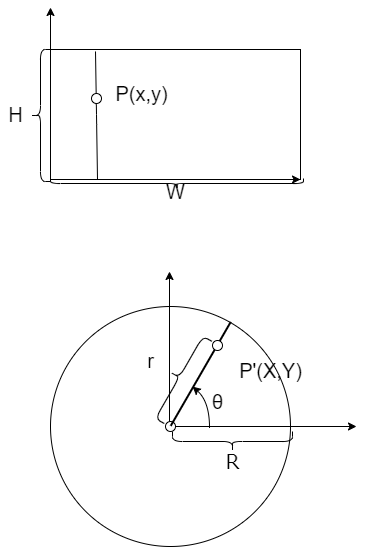
\includegraphics[scale=1.0]{fig/convertintocircle.png}
  \caption{正距円筒図から正距方位図への変換}
\end{figure}

縦$H$,横$W$の大きさで表された正距円筒図の点$P(x,y)$が
半径$R$の正距方位図で点$P'(X,Y)$に写されるとすると,以下の関係式が成り立つ.


\begin{eqnarray}
  \theta = \frac{2\pi x}{W}  \nonumber \\
  r = \frac{Ry}{H} \nonumber \\
  X = r\cos{\theta} \nonumber \\
  Y = r\sin{\theta} \nonumber
\end{eqnarray}

この関係式を用いることで,全天球ビデオカメラで撮影した
パノラマ画像を,glomal350で投影するための正距方位図法を用いた
画像へと変換することが出来る.

\subsection*{GUIの構築}
アプリケーションを操作しやすいようにGUIを構築した.
GUIの構築には,pythonのライブラリであるTkinterを用いた.

Tkinterでは,他のGUIアプリケーション制作ライブラリと同じように,
ボタンや画像などを表示させることが出来るほか,画像にカーソルを重ねたときに
発生するイベント等を登録することができる.今回は,顔をクリックすると
画像が平行移動する処理や,実験の解析のために操作のログを残すために使用した.

\chapter{実験}
%\section{本章の概要}
\section{実験の目的}%・OEBと4章で紹介した視線情報共有手法を用いて,一人が多人数に対しプレゼンテーションを行う際,被検者がどのように感じたかを定性的に調べる

%・意図した視線が正確に伝わっていたか,定量的な評価も行う

%・定量的データとアンケート結果から,本システムの優れた点と改善すべき点を明らかにし,今後の研究へとつなげる

OmniEyeBall及び,4章で紹介した視線共有手法を用いて,1人が多人数に対しプレゼンテーションを行う際に
被検者がどのように感じたかを定性的に調べるのが本実験の目的である.

一方で,意図した視線が正確に伝わっていたかを,視線情報の履歴から算出し,定量的な評価も行う.

定量的データとアンケート結果から,本システムの優れた点と改善すべき点を明らかにし,今後の研究へとつなげる.
\section{実験用アプリケーション}%・(4章と重複?要修正)

%・画面のレイアウトについて詳しく記述する

\begin{figure}[tp]
  \centering
  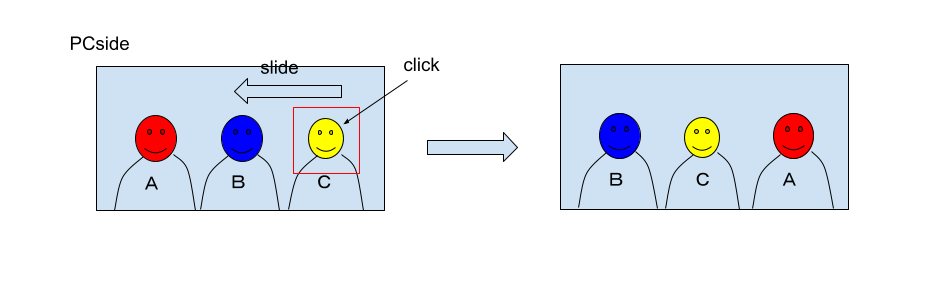
\includegraphics[scale=0.7]{fig/OEBimgSlide.png}
  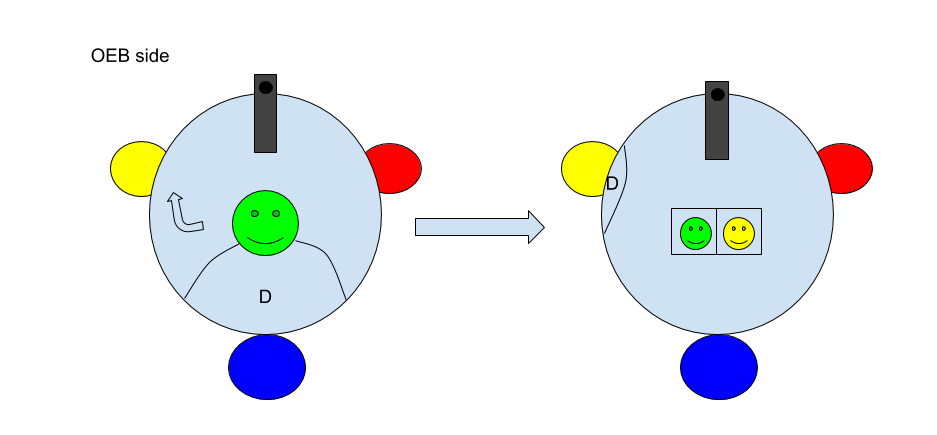
\includegraphics[scale=0.7]{fig/PCimgSlide.png}
  \caption{画像が移動する模式図}
\end{figure}

\section{実験手順}
  \subsection{実験設定}
%・プレゼンター1人,傍聴者3人によるプレゼンテーションを行った

%・プレゼンと質問時間合わせて10分程度

%・提案アプリケーション+OEB使用時と,Zoomのみを使用した場合の2度行った

%・プレゼンター負担削減のため,プレゼン資料は事前に作成した(2種類)

%・また,各傍聴者に,最低一回の質問機会を設けるため,各プレゼンに対し3つの質問項目を事前に用意した

%・実験環境は以下の通り

%・共通:THETA VとTHETA Sを使用,プレゼンターは全天球カメラに対し30cmほど離れていた,プレゼンターのPC詳細(後で調べる)

%・Zoom使用時:質問者側はMac book pro(栗岡机上:後で詳しく)を使用(横に3人並んで一つの画面を見た)

%・OEB使用時:質問者側はOmniEyeBallを使用

プレゼンター1人,傍聴者3人によるプレゼンテーション実験を行った.

プレゼンテーション,及び質疑応答の時間合わせて10分程度の時間を設けた.

従来の平面ディスプレイでの表示を用いた実験,及び5-2節で説明したアプリケーション
を用いた実験の2通りを行った.本来はカウンターバランスをとるため,逆順で2回行う予定だったが,
コロナ感染対策のため参加人数を最小限に抑える必要があり,今回は1回での実験となった.

プレゼンターの負担の削減のため,プレゼンテーションのための資料は事前に作成した.
2通りの実験のため,2種類の資料が存在する.プレゼンテーションの内容は,
SNS用の宣材写真として東京工業大学の敷地内で何を写真に撮るのか,という題で
本館,または図書館を紹介するという物であった.

\begin{figure}[tp]
  \centering
  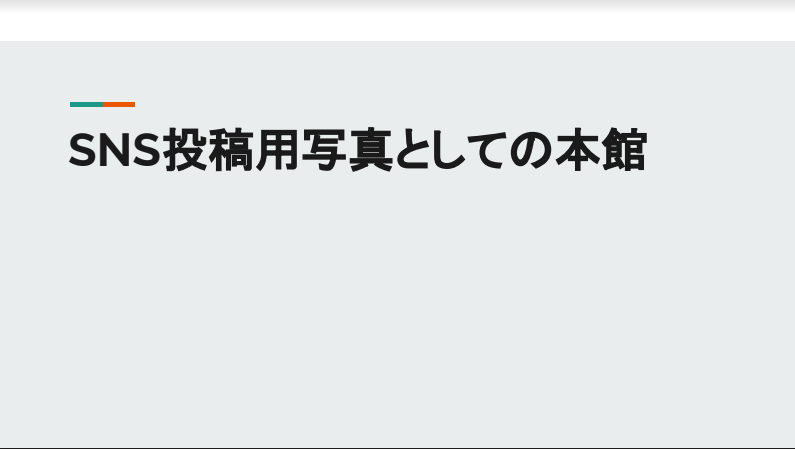
\includegraphics[scale=0.8]{fig/slide1.png}
  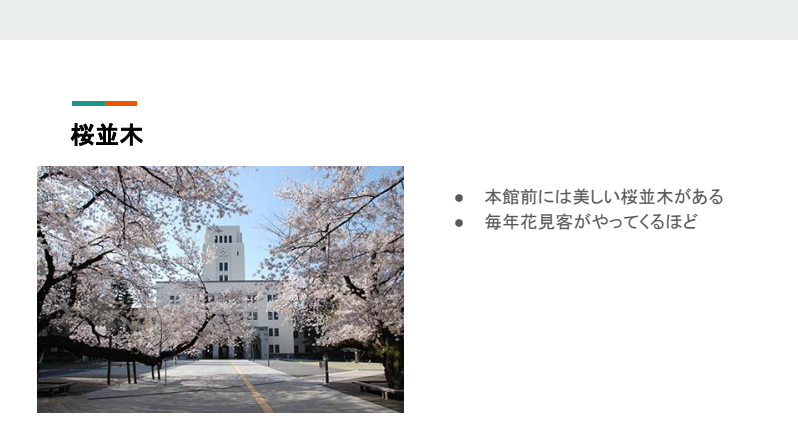
\includegraphics[scale=0.8]{fig/slide2.png}
  \caption{プレゼンターに用意したスライドの一部}
\end{figure}

また,各傍聴者には,それぞれ最低1回の質問機会を設けるため,各プレゼンテーション
に対して3つの質問項目を事前に用意した.

実験環境は以下の通りであった.

\begin{itemize}
  \item プレゼンターの全天球カメラとしてTHETA S,傍聴者側にはTHETA Vを用いた
  \item プレゼンターと傍聴者は全天球カメラからそれぞれ約40cm,50cmほど離れていた
  \item (プレゼンターと傍聴者側で用いたPCの詳細を後で書く)
  \item 傍聴者は平面ディスプレイを使用する際は,PCの前に設置した全天周カメラの前で横に並んで座っていた
  \item また,OmniEyeBallを使用する際は,120°の間隔で,球状ディスプレイを囲んで座っていた
\end{itemize}



  \subsection{実験項目}・定量的な項目と定性的な項目それぞれ設けた

・以下定量的項目

・プレゼンター側が誰を見ていたのかをリアルタイムで記録

・同時に,質問者側は,目が合っていると感じる間,キーを押しっぱなしにして時間を記録

・見ているときに目が合ったと感じた割合(真陽性率)

・見ていないのに目が合ったと感じた割合(偽陽性率)を算出

・以下定性的項目

・System Usability Scale に基づいた5段階評価項目10個

・独自の評価項目(5段階評価2つ+記述式項目)

・OEBを使用したケースとPCを使用したケース両方を経験した被検者に対し,どちらの方が好ましいかを問う
記述式項目を設けた
  \subsection{被験者の動き}\begin{comment}
・OEB使用時と平面ディスプレイ使用時の2回の実験を行った(プレゼンター1人,質問者3人)

・平面ディスプレイ使用の実験の後,10分程度の休憩時間を設け,OEBを使用する実験に移った

・実験の開始前に,使用するアプリケーションの操作説明を行った

・また,5分程度,事前準備したスライドの内容をある程度覚えてもらった(プレゼン中,出来るだけ映像の方を見てもらうため)

・プレゼンターは,プレゼン中,3つ存在するプレゼン内容のチャックポイントに合わせ,ランダムな順番で1人づつ,対応する被験者を見てもらった

・また,質問中は質問を受けている被検者の方向を見るように指示した

・OEB使用時は,見る被験者の映像をクリックし続けることで,視線情報のログを取った

・平面ディスプレイ使用中は,被検者それぞれに対応したキー(映像に移っている左の人間からA,S,D)を押しっぱなしにしてもらうことで視線情報のログを取った

・一方,質問者側の被験者3人には,プレゼン中はプレゼンを聴くように指示した

・質問は,事前に準備した質問3つをランダムな順番で行った(プレゼンターから質問するように促される)

・上記の質問が終わったのちは各質問者から自由に質問してもらい,プレゼンと質問合わせて約10分使用した
\end{comment}
この節では,実験中の被験者の行動の仔細について述べる.
先述の通り,実験はOmniEyeBall使用時と平面ディスプレイ使用時の2回の実験を行った.
プレゼンターは1人で,傍聴者は3人であった.両サイドは異なる部屋で実験を行い,無線
遠隔通信でのビデオ会議を行った.2実験の間には約10分の休憩を設けた

実験の開始前に,使用するアプリケーションの説明を行った.
プレゼンターには,各傍聴者の周辺をクリックすると傍聴者が正面にくること.
及び,OmniEyeBallでどのように映像が表示されるかを伝えた.一方で
傍聴者側には,自身が見られていると全天球カメラに映ったプレゼンターが
個人の方向を向くこと,それ以外の状況では画面上部に小窓が表示されることを
伝えた.

一方で,プレゼンテーションや質問についても一定の指示を行った.
プレゼンターに対しては,プレゼンテーション前に,出来るだけ
カメラの方向を見てもらえるように,事前準備したスライドの内容を
5分ほど眺めてもらい,大筋を把握するように指示した.
また,準備した資料には3つのチェックポイントを設けて,その
部分を読み上げるタイミングで,ランダムな順番で1人毎,傍聴者を
見るように指示した.質問中は,質問を受けている傍聴者の方向を
見るように指示した.さらに,誰を見ていたかをリアルタイムで記録するために
追加の操作を行ってもらった.OmniEyeBall使用時は,見ている傍聴者の
映像をクリックし続けるように,平面ディスプレイ使用時は,傍聴者それぞれに
対応したキーボードのキーを押し続けてもらうことで視線情報の履歴を
録った.

傍聴者側には,タブレット端末を渡し,
プレゼンターの紹介するプレゼン資料を事前に
配布し,プレゼンテーション中にいつでも参照できるようにした.
プレゼンターのプレゼンテーション中には,資料を好きに参照しながら
傍聴してもらうように指示した.質疑応答の時間には,事前準備した
質問3つをランダムな順番で1人1つづつ問うようにしてもらい,その後は
自由に質問するように指示した.定量的評価のため,プレゼンターを目が
合ったと感じている間は,指定のキーを押し続けてもらうように指示した.

\begin{figure}[tp]
    \centering
    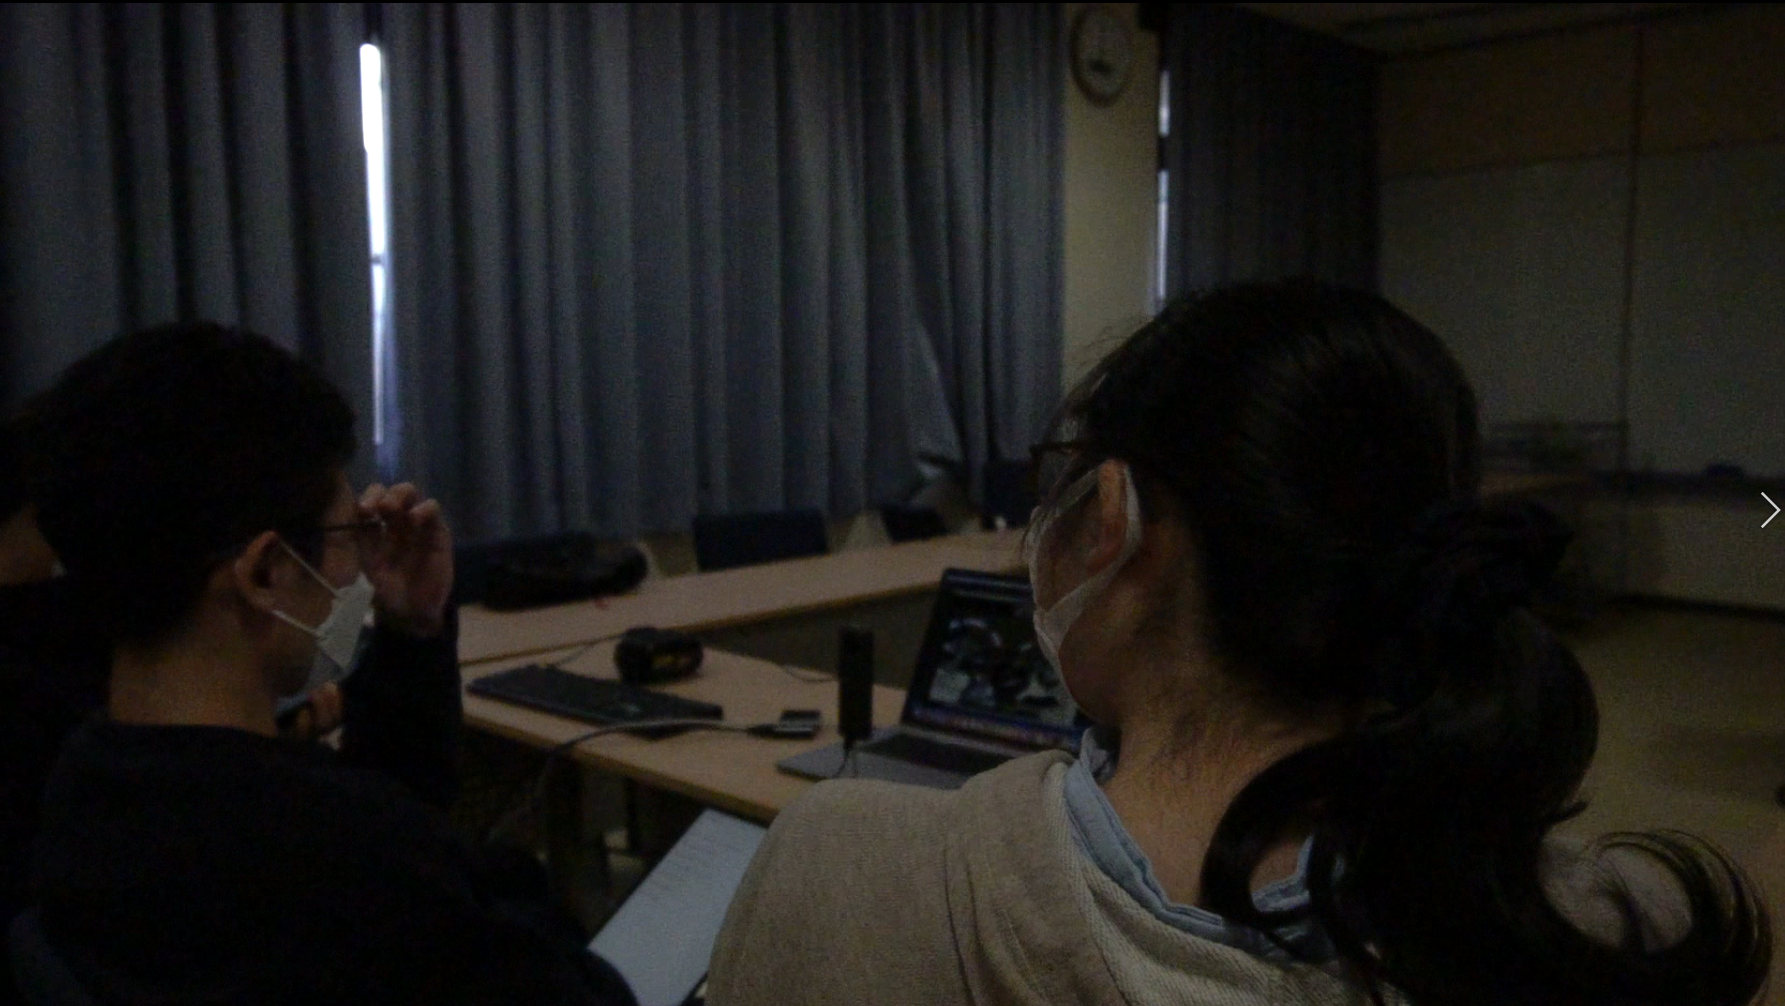
\includegraphics[scale=0.2]{fig/exp1.png}
    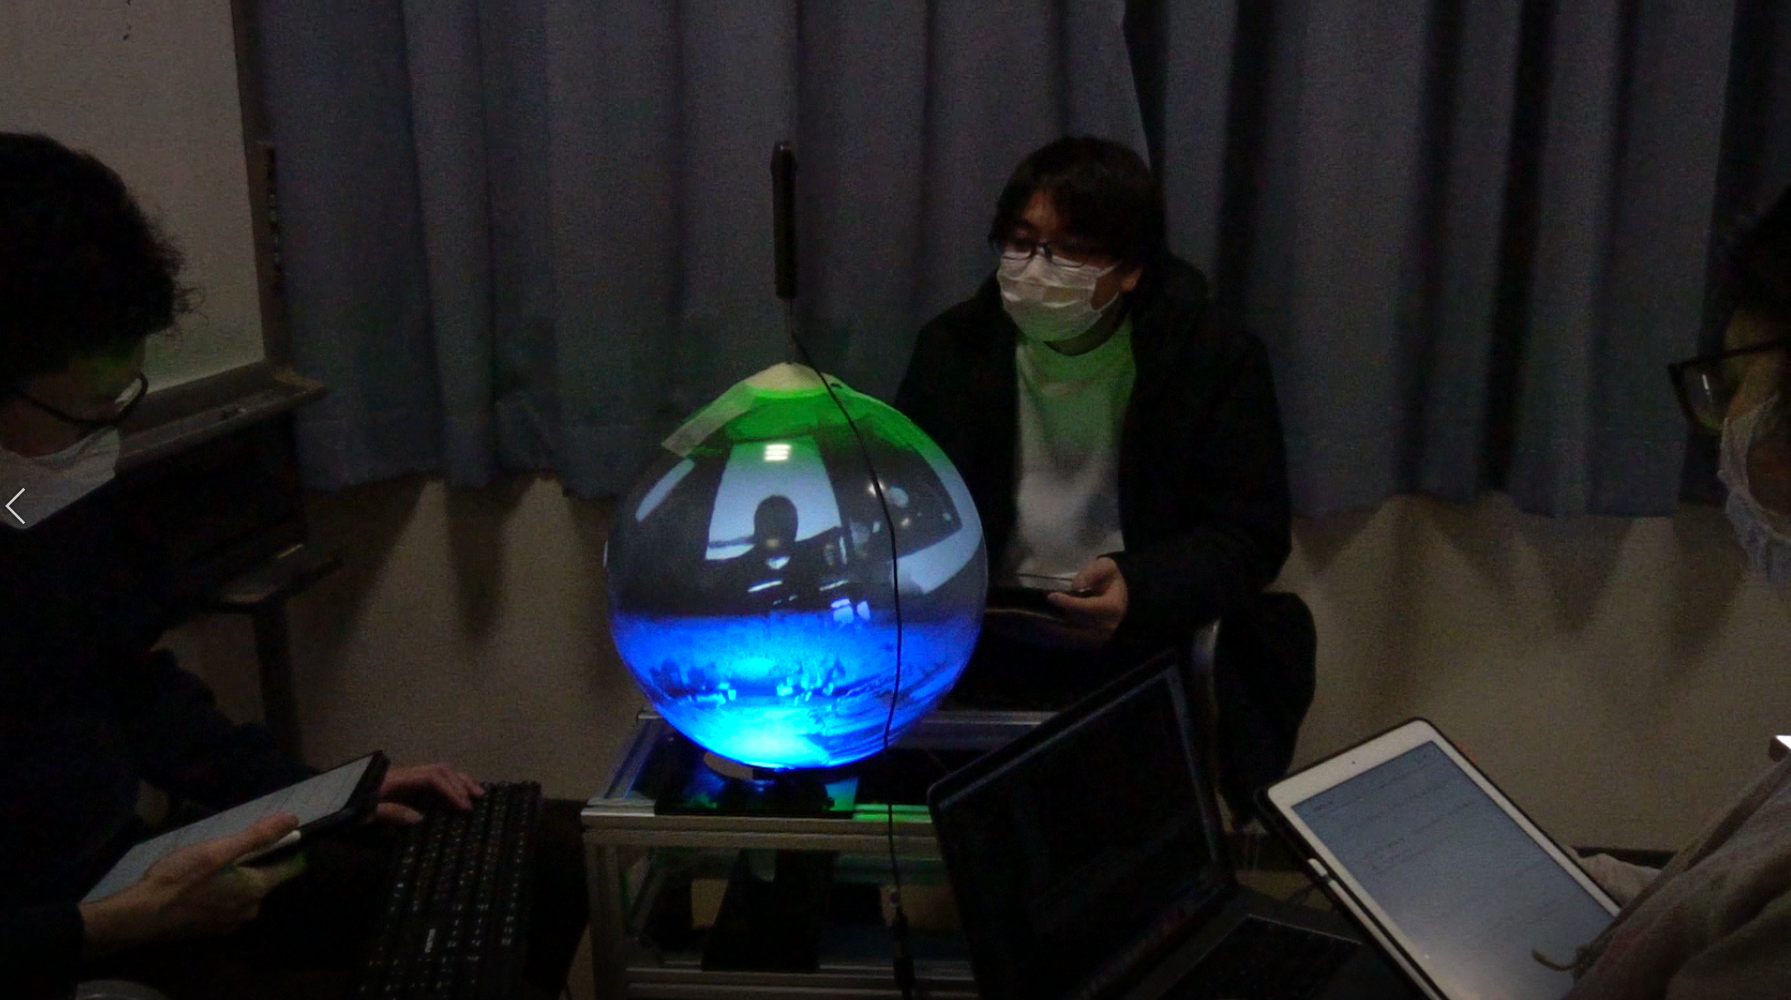
\includegraphics[scale=0.2]{fig/exp2.png}
    \caption{傍聴者側の実験の様子}
\end{figure}

\begin{figure}[tp]
    \centering
    \includegraphics[scale=0.2]{fig/exp4.png}
    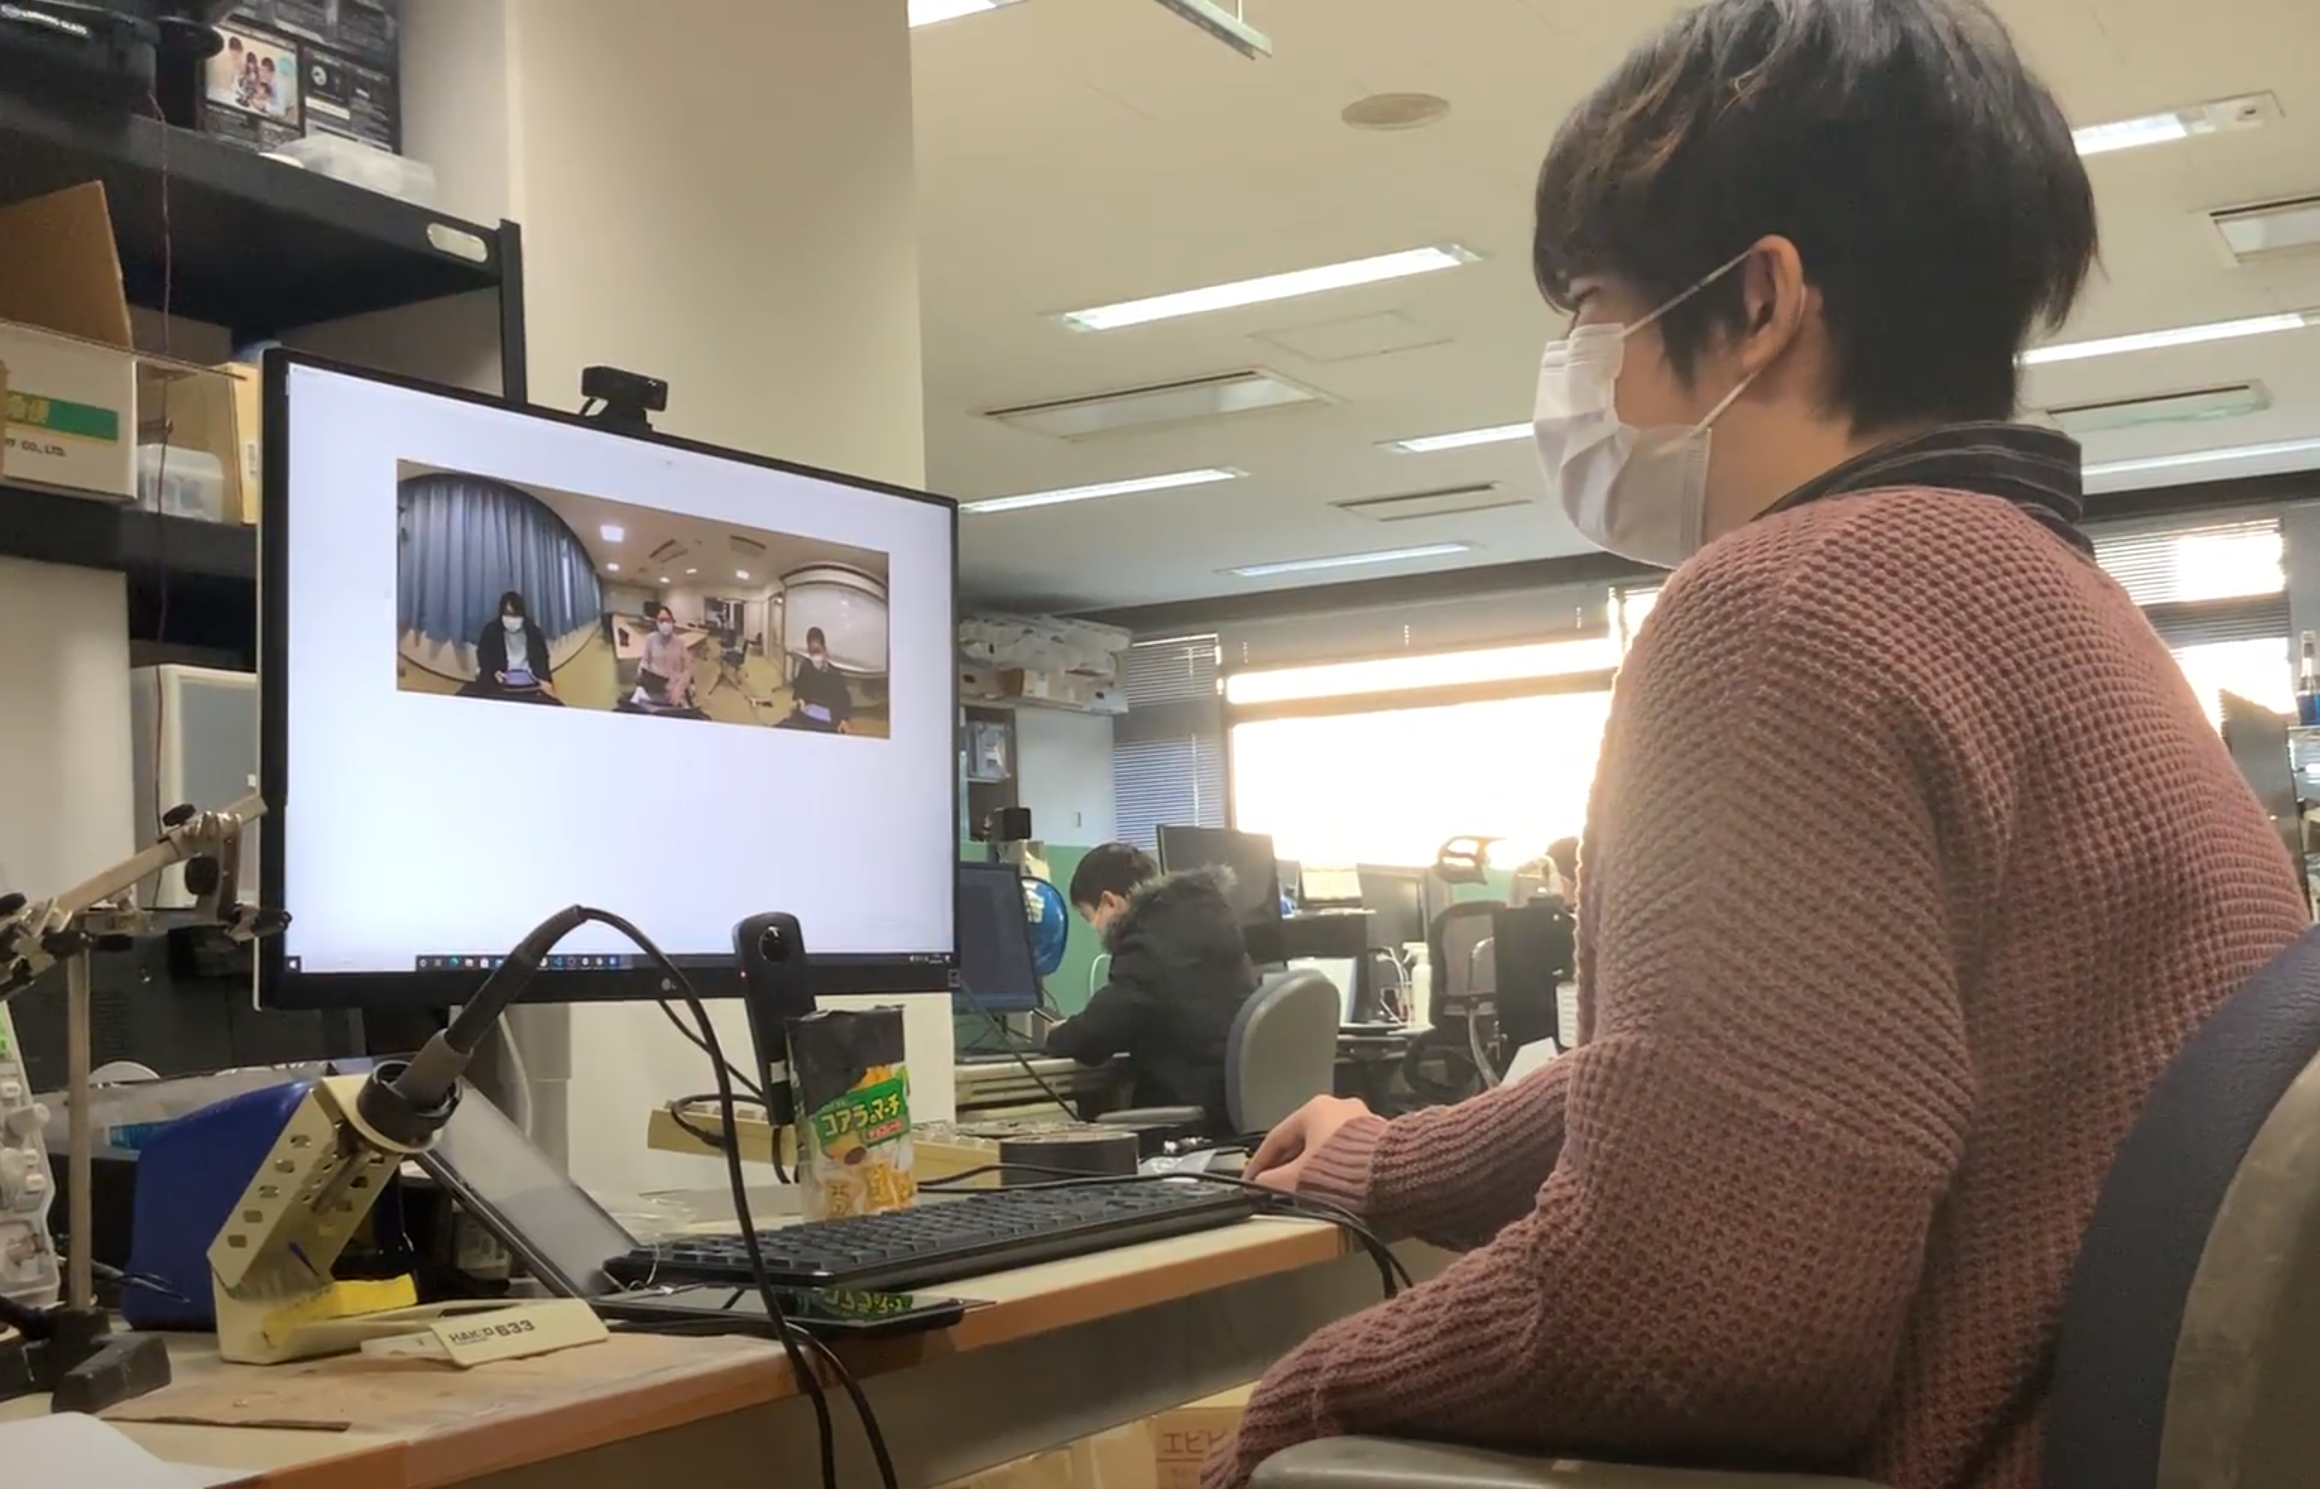
\includegraphics[scale=0.2]{fig/exp3.png}
    \caption{プレゼンター側の実験の様子}
\end{figure}
\section{実験結果}
  \subsection{定量的評価}定量的評価の結果を以下に示す.

\begin{table}[tp]
  \begin{center}
  \begin{tabular}{|c|c|c|}
  \hline
       & 真陽性率 & 偽陽性率 \\ \hline
  被検者1 & 0.05 & 0.02 \\ \hline
  被検者2 & 0.57 & 0.12 \\ \hline
  被検者3 & 0.00 & 0.00 \\ \hline
  \end{tabular}
  \caption{平面ディスプレイ使用時}\label{rate1}
\end{center}
\end{table}

\begin{table}[tp]
  \begin{center}
  \begin{tabular}{|c|c|c|}
  \hline
       & 真陽性率 & 偽陽性率 \\ \hline
  被検者1 & 0.06 & 0.07 \\ \hline
  被検者2 & 0.87 & 0.28 \\ \hline
  被検者3 & 0.19 & 0.00 \\ \hline
  \end{tabular}
  \caption{OEB使用時}\label{rate2}
\end{center}
\end{table}

  \subsection{定性的評価}定性的評価の,5段階評価項目の結果は以下の通り.
記載した箱ひげ図については,左から質問1から12の順に並んでいる.
\begin{figure}[tp]
  \centering
  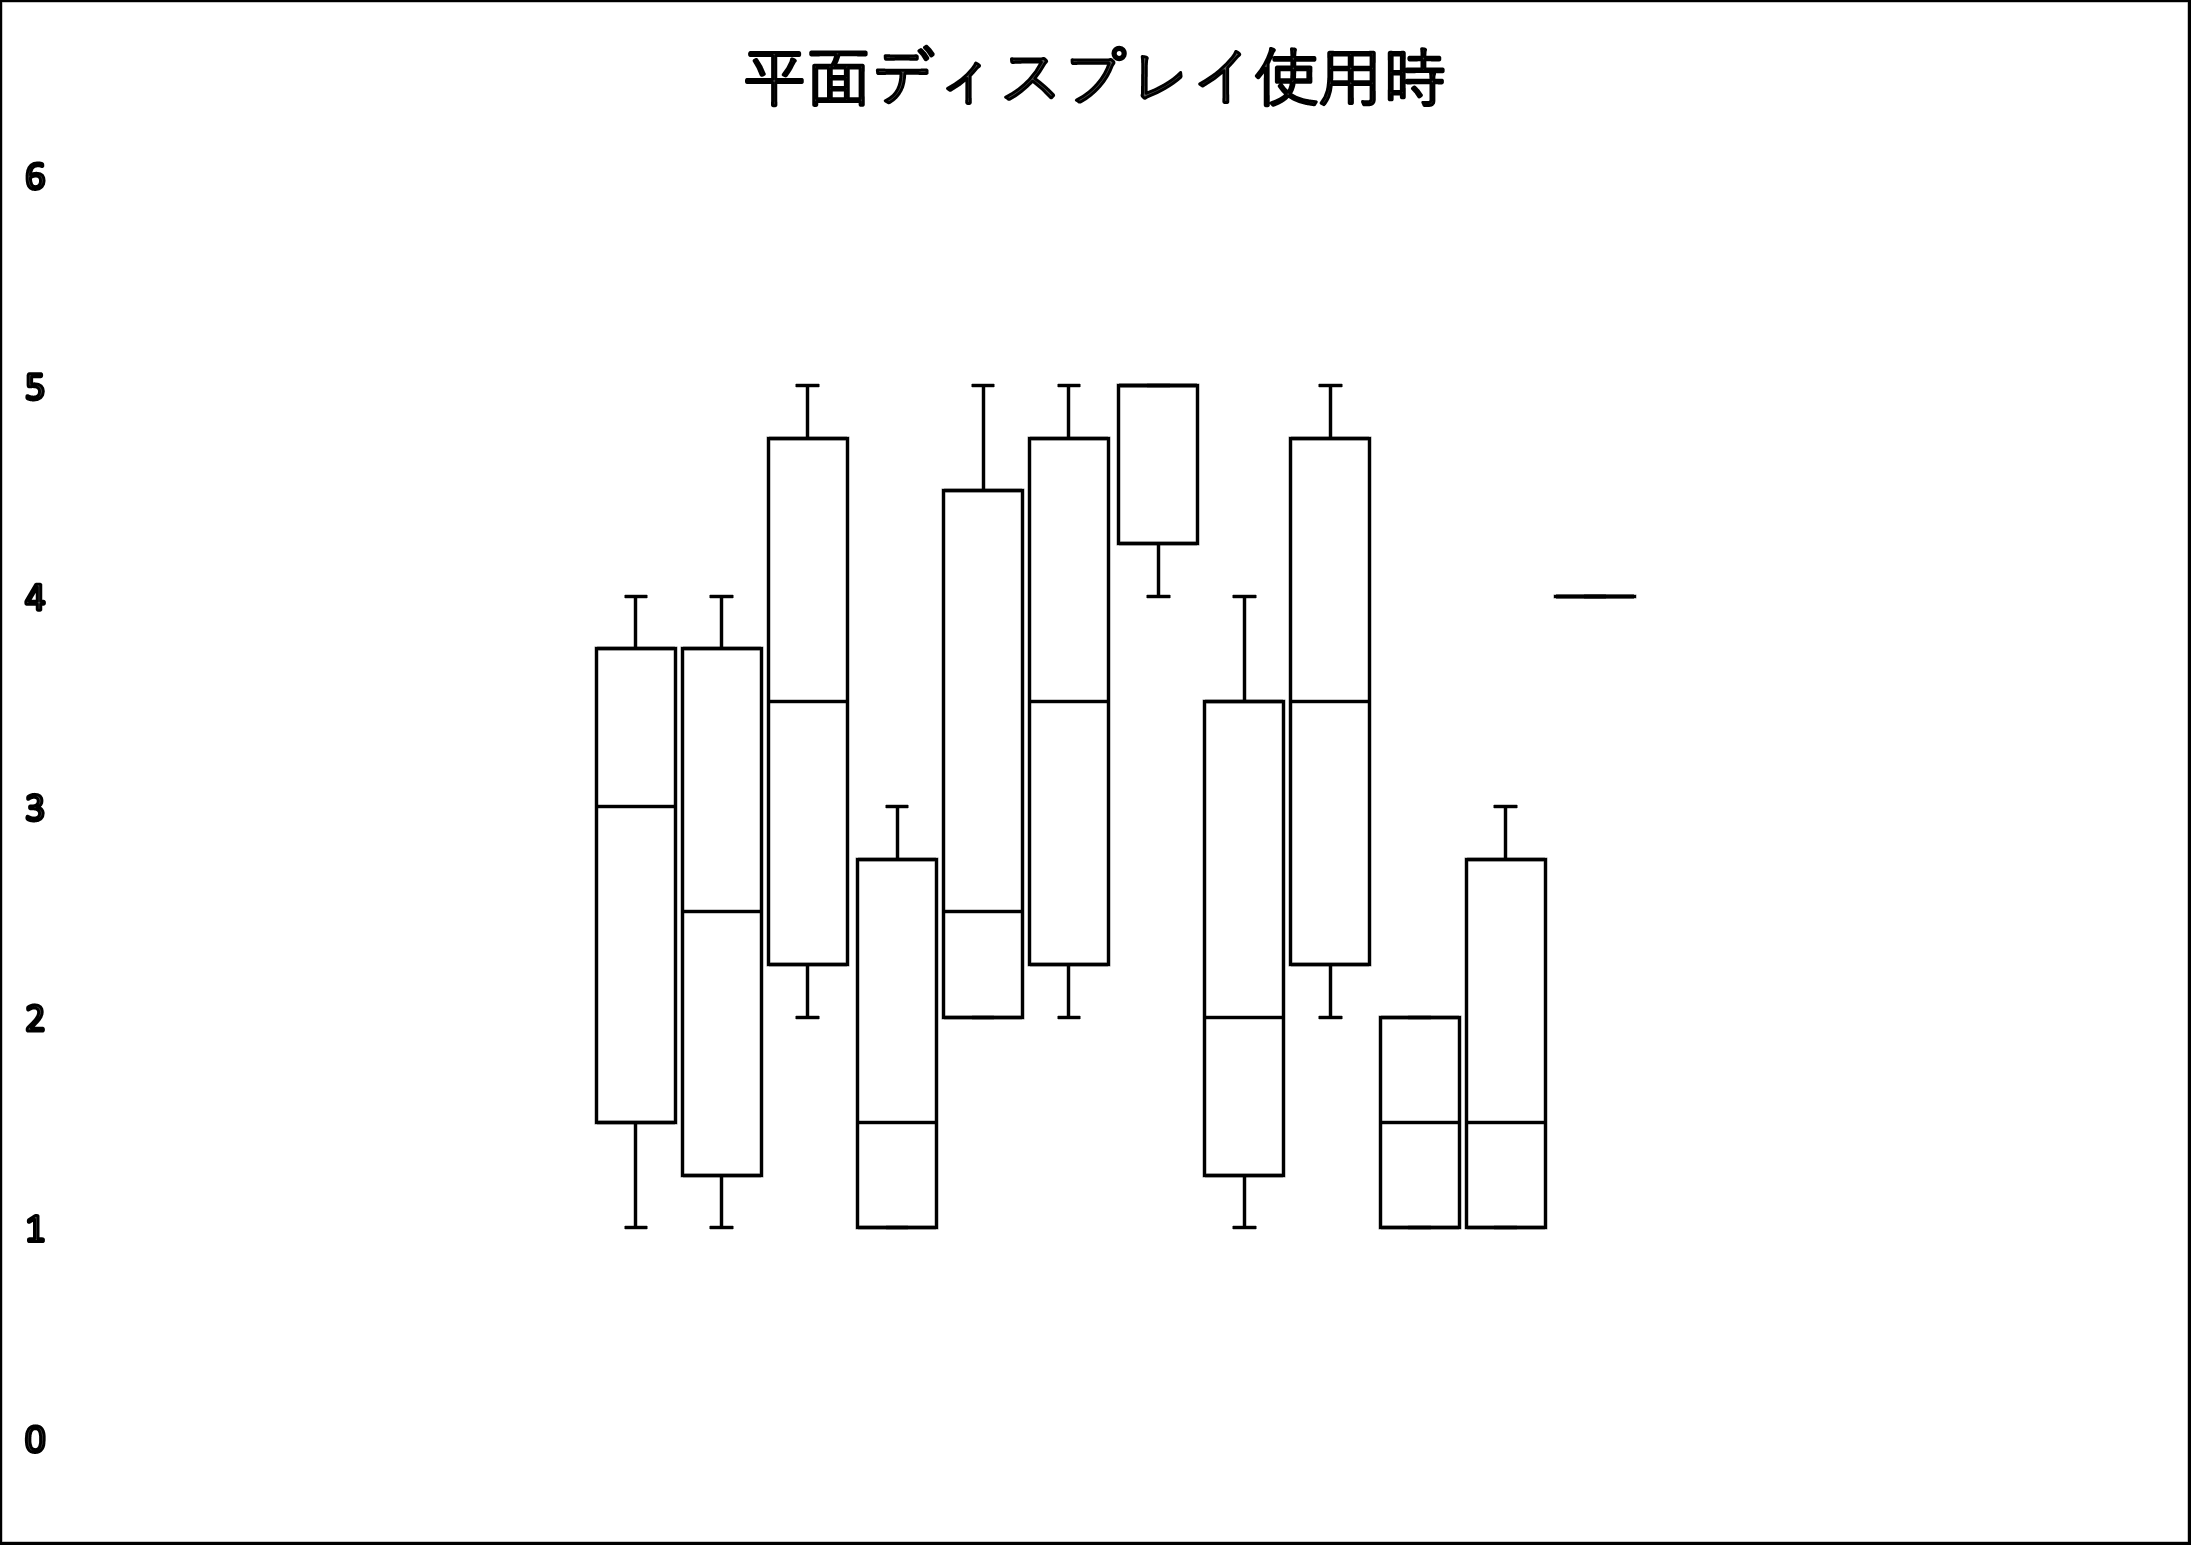
\includegraphics[scale=0.9]{fig/boxplot1.png}\label{boxplot1}
  \caption{平面ディスプレイ使用時の5段階評価項目結果}
  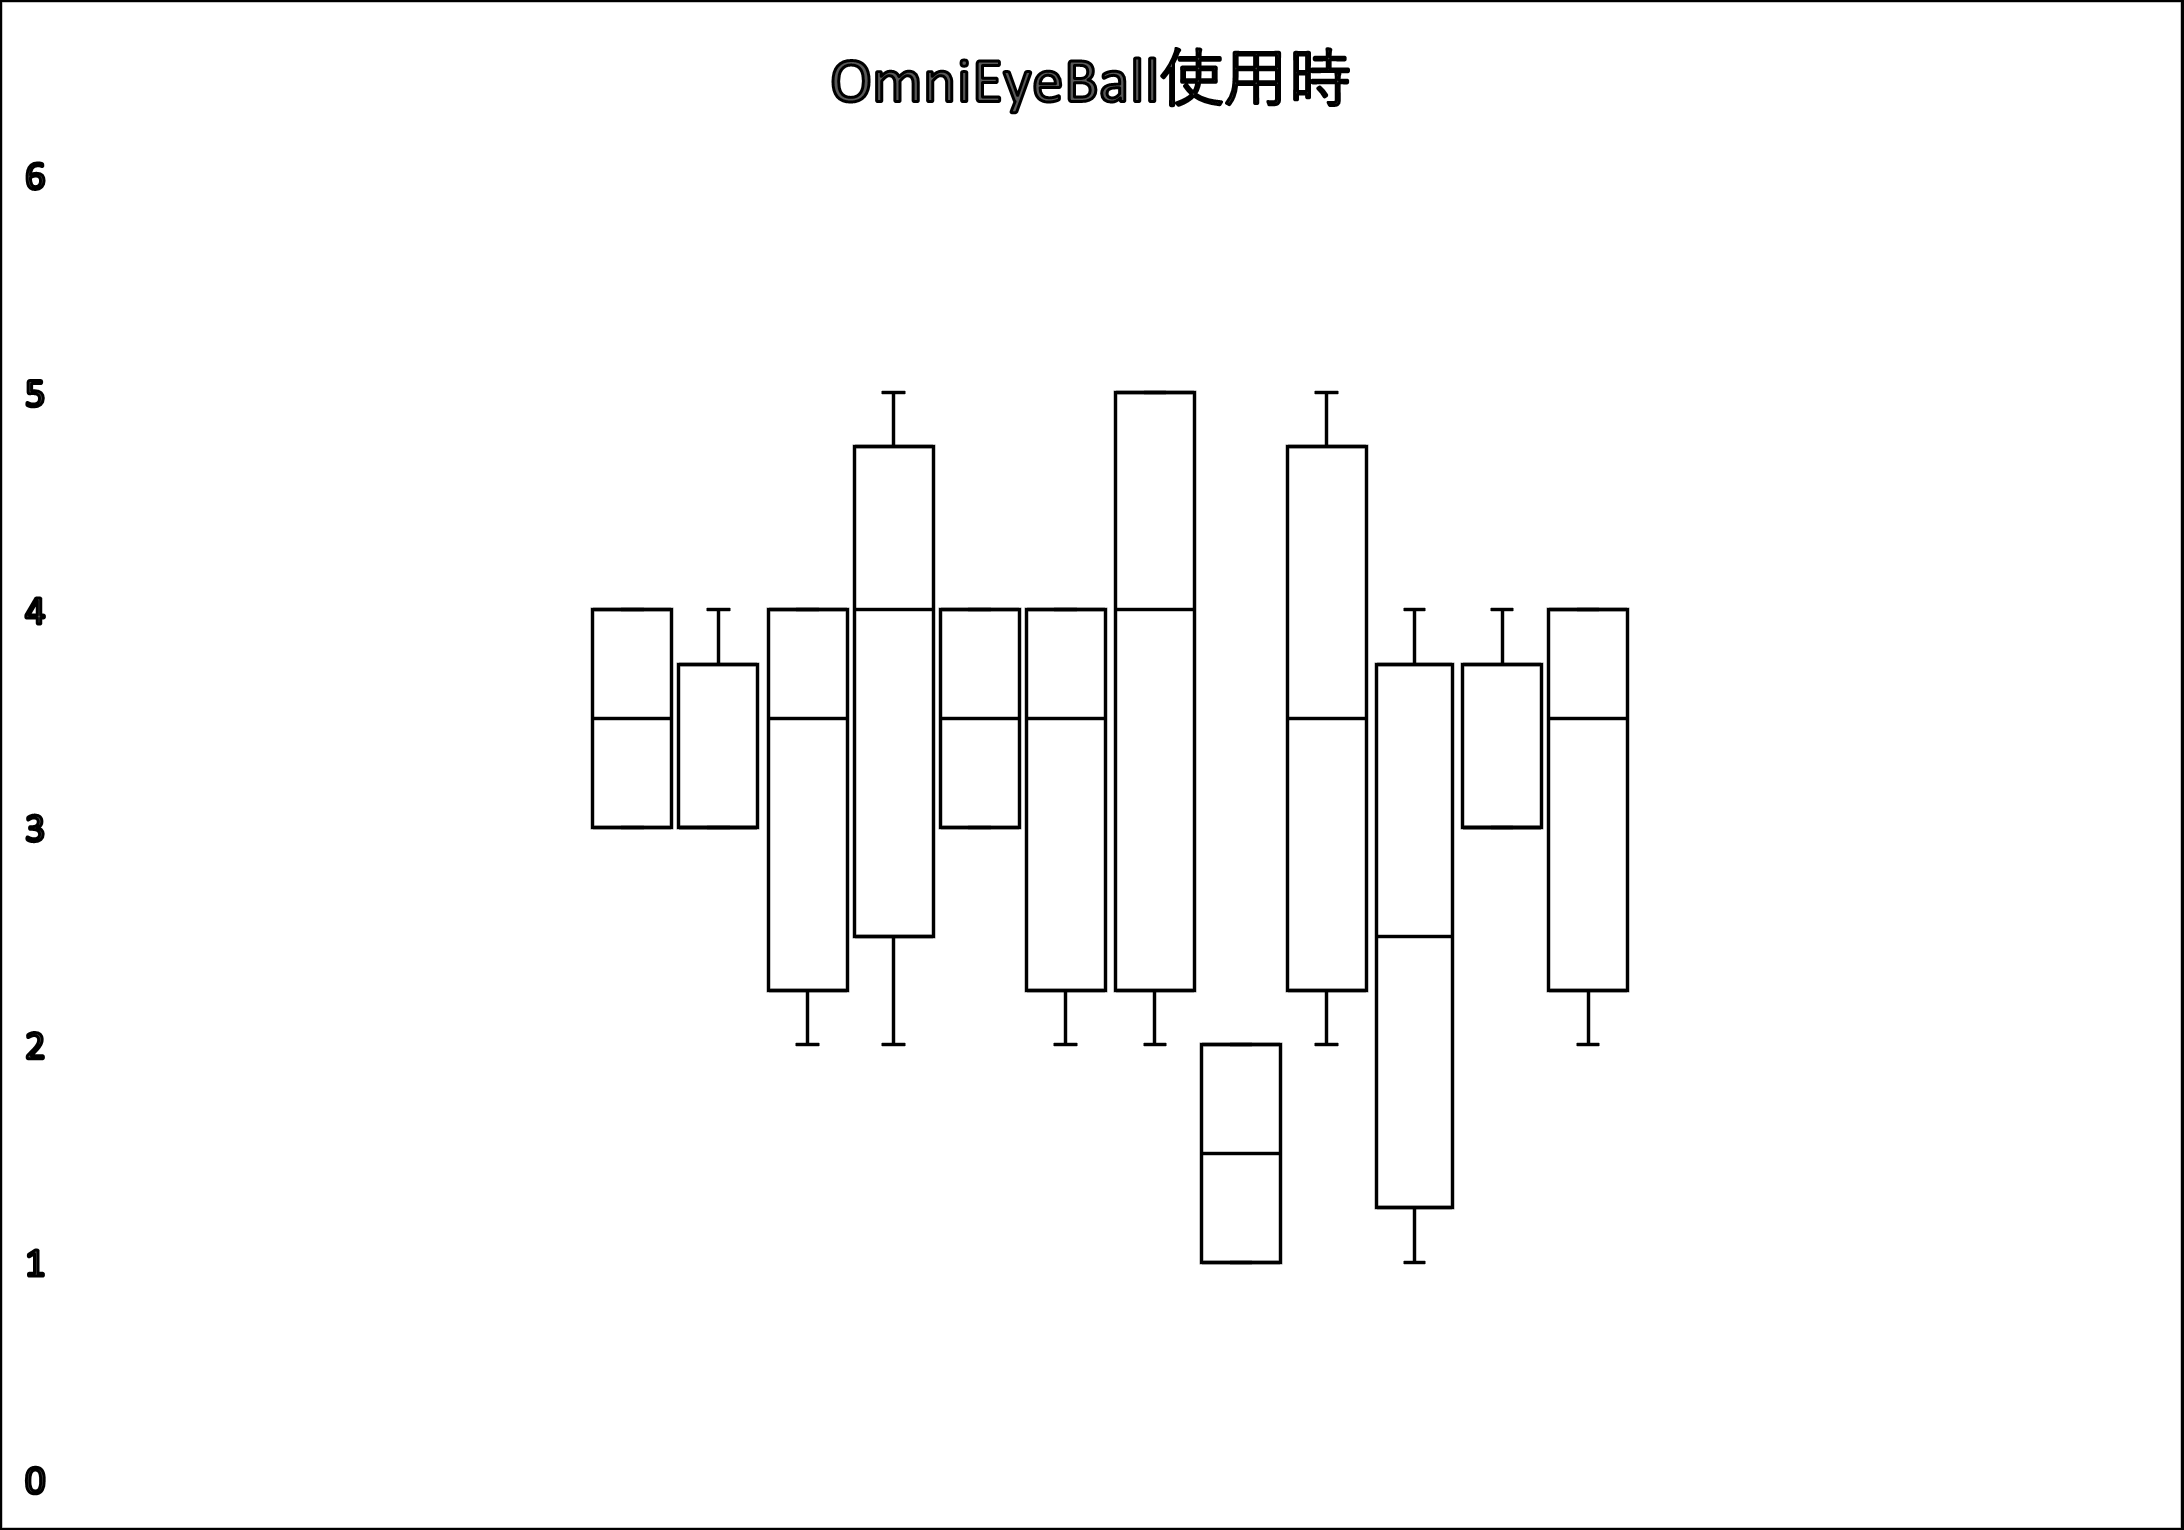
\includegraphics[scale=0.9]{fig/boxplot2.png}\label{boxplot2}
  \caption{OmniEyeBall使用時の5段階評価項目結果}
\end{figure}



\begin{table}[tp]
  \begin{center}
  \begin{tabular}{|c|c|c|}
  \hline
       & 平面時  & OEB時 \\ \hline
  質問1  & 2.75 & 3.5  \\ \hline
  質問2  & 2.5  & 3.25 \\ \hline
  質問3  & 3.5  & 3.25 \\ \hline
  質問4  & 1.75 & 3.75 \\ \hline
  質問5  & 3    & 3.5  \\ \hline
  質問6  & 3.5  & 3.25 \\ \hline
  質問7  & 4.75 & 3.75 \\ \hline
  質問8  & 2.25 & 1.5  \\ \hline
  質問9  & 3.5  & 3.5  \\ \hline
  質問10 & 1.5  & 2.5  \\ \hline
  質問11 & 1.75 & 3.25 \\ \hline
  質問12 & 4    & 3.25 \\ \hline
  \end{tabular}\label{ave}
  \caption{各質問の4人の平均値}
\end{center}
  \end{table}

記述式項目については5-5節にて言及する.

また,平面ディスプレイを使用したケースとOmniEyeBallを使用したケースの
どちらが好ましいかを問う質問では,前者が好ましいと答えた人数は1人,
後者が好ましいと答えた人数は3人であった.
\section{実験結果から得られる知見と考察}・表5.1,5.2を見るとOEB使用時,平面ディスプレイ使用時共に真陽性率(プレゼンターが見ていた時間の中で,目が合ったと感じた時間の割合)
の最大値,最小値の差が非常に大きい(極端な例は平面ディスプレイ使用時の0.00(一度もキーを押さなかった))

・自由記述意見の1つ「発表者の顔の画像が暗くて小さいため、何となく正面を向いている時に目があっていそうだと感じた。曖昧であり、判断に困った」(平面ディスプレイ使用時)
に見られるように,そもそも「目が合っている」という感覚自体があいまいで,人によって見られていると感じた機会が不ぞろいである原因であると考えられる.

・真陽性率は3人とも平面ディスプレイ使用時に対し,OEB使用後の方が増加している

・サンプル数の少なさ,及び順序効果により,比較はできないが,本実験で使用したアプリケーションによって
視線情報が共有されやすくなったという仮定に対し,一考の余地がある.

・一方で,視線情報を小窓の表示状態などからも判断できるOEB使用時の方が,偽陽性率が下がると予想していたが,
2者はOEB使用時の方が偽陽性率が増加した.特に,被検者2の偽陽性率は0.16上昇し0.28となっている.

・「正面に発表者がいて、さらに窓に発表者がいることに違和感を感じました。」(OEB使用時)という意見があった.
本アプリケーションは,「特定の個人を見ていない場合,全員に小窓を表示する」という仕様になっている.
この仕様では,前回の人物クリックの結果,質問者側でプレゼンターの顔が正面に移動したのにもかかわらず,その上に小窓を表示され
2つの顔が映ってしまう.そのため,見られていない時も見られていると錯覚した可能性がある.

・OEBを使用する場合において,上記以外にも小窓の表示方法に関する意見が多くみられた.

・「顔の切り抜きはもう少し下に置くことは可能か?」

・「OEBについての説明が少ないので仕様がよく分からなかった。小窓がなくなった時がよくわからなかった。小窓が唐突に消えるのに驚いた。」

・よって,小窓の表示方法に関しては再考する必要がある.

・また,全天球ビデオカメラにおいて,被写体の顔が小さく表示されるという意見も多くみられた.

・「3人のうち誰か一人を見るということが難しいと感じた(視野に全員が収まっているので誰か一人にフォーカスして話しづらい)」

・「顔とカメラが遠い?からなのか、そもそも目が見えなかった」

・「発表者の顔の画像が暗くて小さいため、何となく正面を向いている時に目があっていそうだと感じた。曖昧であり、判断に困った。」(いずれも平面ディスプレイ使用時)

・全天周カメラ自体の視野の広さと,撮影領域上下が広がるような歪みによって,相対的に顔が小さくなることが原因であると考えられる.

・よって,全天周カメラを用いて顔を映したコミュニケーションを行う際には,何らかの方法で顔部分をクローズアップする必要がある.

・「ディスプレイのサイズ的に3人とも常に視野の中に収まってはいるので、クリックした人が真ん中に来る必要はないかな…と感じた。
画像そのものが移動するよりは、クリックしている間はカーソルの周辺に枠がでる…とかのほうが「ひとりにフォーカスしている感」があって良いかもしれないと思いました。」(OEB使用時,プレゼンター側)

・PCを使用するプレゼンター側において,常にカメラの方を向くことで見たい人間を正面に捉えるように設計したが,常に3人とも視界に入っているためかえって混乱を招くことになった.


\chapter{考察}
%\section{本章の概要}
\section{本システムの問題点}\begin{comment}
・また,SUSのネガティブな評価項目がOEB使用時で有意差は見られないものも,5に近くなってしまっている.

・OEB使用時のアンケート結果でGUIに関する意見が多く出ている.

・特に「仕様が分かりづらい」,「小窓の表示位置を変えたい」という趣旨の意見が多くみられた.

・小窓の位置のみならず,本来の全天球カメラの映像に被さって小窓が表示される仕様など,映像が複雑になってしまう状況もあり,
それが混乱を招いた可能性がある.

・また,全天球カメラ自体の視野の広さから,パノラマ映像では顔が小さく表示されやすく,PCの画面に表示する
全天周カメラの映像表示方法にも改善の余地がある.

・算出した偽陽性率に改善が見られなかった点から,小窓に表示する顔の表示方法自体も変更する余地がある.

・実験結果に関係しない事項としては,実験用アプリでは被験者の位置が変更しない制限があったが,
実際は被写体は自由に動くことが出来るべきである.被写体が移動しても正しく小窓を表示できるように
する必要がある.
\end{comment}
5章で,立体的な映像から,対面しているかのような感覚を得やすいという結論
が得られた.これに基づいて,実際に対面した時に見えるような立体視を
再現することが効果的であると考えられる.6章ではより立体感のある
小窓の表示方法や,全天球カメラの映像の表示方法を組み込んだアプリケーションを
提案する.

加えて,小窓の表示位置の改善を行う.そうすることで,よりユーザーに対して
分かりやすい映像の表示方法を提案する.

実験結果に関与しないが,改善すべき点として,実験と違い
被写体が移動するという条件が加わる.被写体が移動しても
動的に小窓の表示位置を変更できるように,顔認識ライブラリを
用いた手法を組み込む.

\section{本システムの応用}
  \subsection{対話相手表示形式}%・6-2-1~3節では小窓の表示方法,あるいは顔自体の表示方法などを変更したアプリケーションを提案する

%・まず,実験用アプリケーションと同様に,

\begin{comment}
\begin{itemize}
  \item 6-2-1~3節では小窓の表示方法,あるいは顔自体の表示方法などを変更したアプリケーションを提案する
  \item まず,実験用アプリケーションと同様に,小窓に,PC使用者と,見られている参加者の2人を表示する手法を提案する
  \item 実験用アプリケーションと異なる点は以下の通り
  \item 小窓の表示位置を,球体ディスプレイの赤道部分に寄せる
  \item 顔認識ライブラリdlibを用いて,顔を認識した位置に対して小窓を表示する
  \item PC使用者は,実験用アプリケーションの時と異なり,指定の位置ではなく可変な被検者の顔の位置をクリックすることで
        被験者を見ることが出来る
  \item 顔を中心に持ってくるのではなく,GUIの空いていた領域(画面下部)にクリックした人物の顔の切り取りを表示する
  \item (dlibについての説明,アプリケーションの様子,クリックした位置に顔を持ってくるプログラムについての説明を行う)
\end{itemize}
\end{comment}

この節では,小窓にPC使用者と見られている人間の2つの顔を
表示するアプリケーションを提案する.実験用アプリケーション
との変更点は以下のとおりである.
\begin{itemize}
  \item 小窓の表示位置を,球体ディスプレイの赤道部分に寄せる
  \item 顔認識ライブラリDlib\cite{12}を用いて,顔を認識した位置に対して小窓を表示する
  \item PC使用者は,実験用アプリケーションの時と異なり,指定の位置ではなく可変な
  被験者の顔の位置をクリックすることで被検者を見ることが出来る
  \item 顔を中心に持ってくるのではなく,GUIの空いていた領域(画面下部)にクリックした人物の顔部分を表示する
\end{itemize}

変更点の1つ目は
\begin{itemize}
  \item 顔の切り抜きはもう少し下に置くことは可能か?
\end{itemize}
という,被検者からのコメントに対しての実装である.実際に,
正距円筒図法によって出力された全天球パノラマ画像に,正方形で切り取った
顔部分の画像を張り付けると,歪みを考慮していないために,上部分ほど
実際より小さく表示されてしまうという問題がある.
例えば緯度60°に相当する部分は,正距円筒図法上では赤道と同じ長さであるが
球体ディスプレイ上では赤道の長さの半分になってしまう.(表\ref{projection1}参照)よって,歪みの
影響の少ない球体ディスプレイの赤道近くに顔の小窓を表示することが適切であると
考えた.
\begin{figure}[tp]
  \centering
  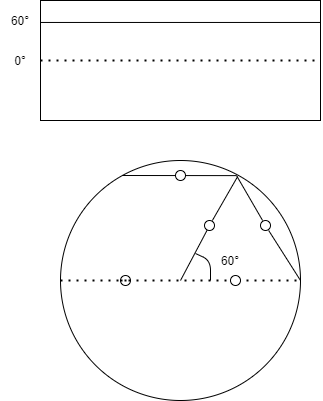
\includegraphics[scale=0.7]{fig/projection1.png}\label{projection1}
  \caption{上部分が縮小して表示される様子}
\end{figure}

変更点の4つ目は
\begin{itemize}
  \item ディスプレイのサイズ的に3人とも常に視野の中に収まってはいるので、クリックした人が真ん中に来る必要はないかな…と感じた。画像そのものが移動するよりは、クリックしている間はカーソルの周辺に枠がでる…とかのほうが「ひとりにフォーカスしている感」があって良いかもしれないと思いました。
  \item 3人のうち誰か一人を見るということが難しいと感じた(視野に全員が収まっているので誰か一人にフォーカスして話しづらい)
\end{itemize}
というプレゼンターからのコメントを反映させた.
また,顔にフォーカスし,表示させることで,全天球カメラの視野の広さによって
顔が相対的に小さく見えてしまう問題の解決も目指した.

\subsection*{Dlib}

\begin{figure}[tp]
  \centering
  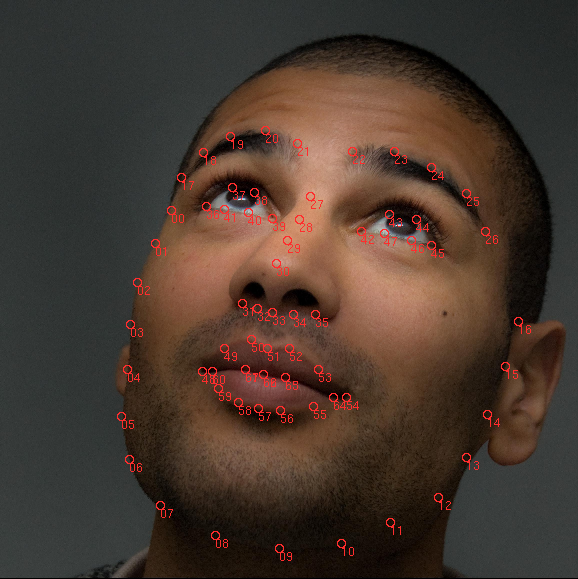
\includegraphics[scale=0.7]{fig/dlib.png}
  \caption{Dlibの顔検出} \cite{13}
\end{figure}

顔認識には,C++やpythonで利用可能な,クロスプラットフォームソフトウェアライブラリ
であるDlibを用いた.Dlibには様々な種類の顔認識モデルが事前に準備されている.
代表的なものを以下に示す.
\begin{itemize}
  \item HOG(Histograms of Oriented Gradients)+SVN(Support Vector Machine)
  \item CNN
\end{itemize}

\subsubsection*{HOG+SVN}
HOGは局所領域の輝度の勾配を
求め,ヒストグラム化した特徴量である.画像はブロックと呼ばれる局所領域
に分割され,さらにブロックはセルと呼ばれる局所領域に分割される.セル毎に
各ピクセルの輝度勾配を計算し,勾配の方向で分類したヒストグラムを作成する.
各セルの各勾配方向におけるヒストグラムは,ブロック内のヒストグラムの総和に
よって正規化される.

SVNは,データを2クラスに分類するために
最適な超平面を求めるアルゴリズムである.$n$次元空間における超平面は,
次元が$n-1$の平坦な空間であり,元の空間を2つに分割する.

\subsubsection*{CNN}
CNNは,従来のニューラルネットワークに,畳み込み層やプーリング層といった
層を組み合わせて作られるニューラルネットワークである.画像認識の分野では
よく用いられている.

\begin{figure}[tp]
  \centering
  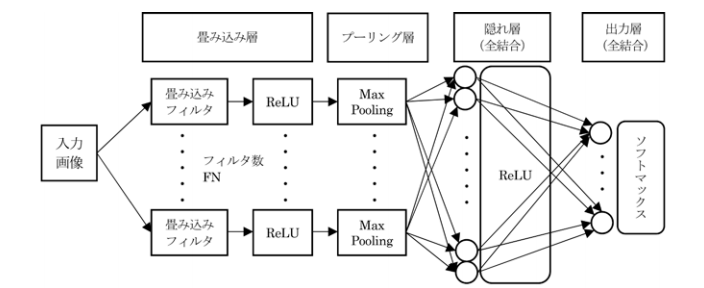
\includegraphics[scale=0.7]{fig/CNNep.png}
  \caption{CNNの一例} \cite{13}
\end{figure}

畳み込み層では,学習可能なパラメータであるカーネル及びバイアスを用いて,入力に対して
畳み込みが行われる.画像データの畳み込みに際しては,ある注目ピクセルと
その周辺のピクセルが出力に用いられることで,画像の空間的な情報が損なわれにくい
という利点がある.

カーネル$K$のサイズが$N*N$であった場合,画像のあるピクセルの周辺$K*K$サイズの
領域$A$にカーネルを適用した結果は,$K$と$A$のアダマール積となる.すなわち

\begin{eqnarray}
  \sum_{i=1}^{N} \sum_{j=1}^{N} k_{ij}a_{ij} \nonumber 
\end{eqnarray}
である.

カーネルを適用する領域は通常1ピクセルずつずらされる.そうして
全ての領域にカーネルが適用され,バイアスを加算した結果が畳み込み層の出力
として用いられる.

\begin{figure}[tp]
  \centering
  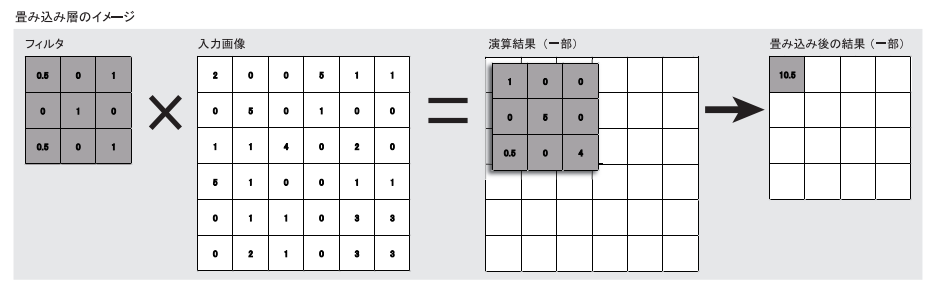
\includegraphics[scale=0.6]{fig/conv.png}
  \caption{畳み込みのイメージ} \cite{14}
\end{figure}

プーリング層は,通常畳み込み層の直後の層であり,畳み込み層の
出力を,カーネルを用いてダウンサンプリングした結果を出力する.

ここで用いられるカーネルは,カーネル適用範囲の平均値を出力するものと,
カーネル適用範囲の最大値を出力するものがよく用いられている.
前者の場合はAverage Pooling層と呼ばれ,後者ならMax Pooling層と呼ばれる.
カーネルの適用範囲のずらし幅はストライドと呼ばれ,様々な値が設定されている.

\begin{figure}[tp]
  \centering
  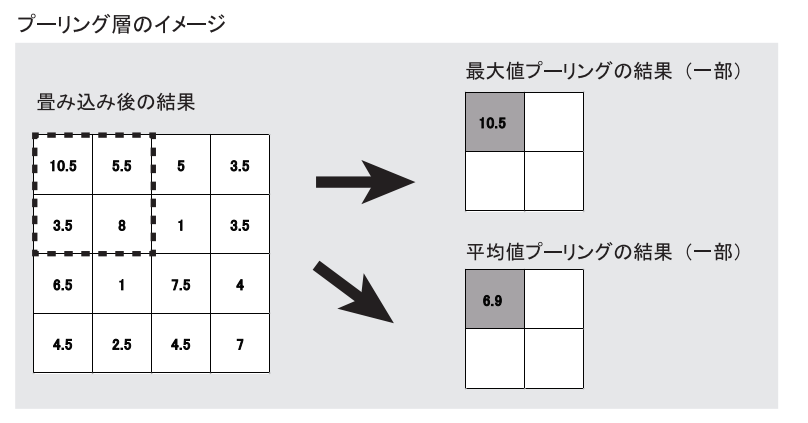
\includegraphics[scale=0.7]{fig/pooling.png}
  \caption{プーリングのイメージ} \cite{14}
\end{figure}

今回のアプリケーションでは,より精度の高いCNNを用いたモデルを使用した.
一方で,HOG+SVNを用いるモデルは,識別実行速度が速いという利点がある.






  \subsection{横顔生成形式}\begin{comment}
\begin{itemize}
  \item 2人の顔をウインドウで表示する代わりに,対面で人の横顔を見るような表示
  \item 横顔を表示することで,立体感を拡張させ,あたかも対面しているかのような状況を作り出す
  \item 今回は横顔の生成は実際の映像を用いては行っていない
  \item Unity上で3Dモデルを横から撮影し,UnityCapture\cite{8}を用いて仮想カメラの映像としてOpenCVで処理した
  \item 後述するおかしら会議\cite{10}のように,Unity内の球体に画像をマッピングして,疑似的に顔を生成し,横から撮影する
  というった方法も考えられる.
  \item 機械学習ベースの横顔生成手法としてYiboら\cite{11}の方法が挙げられる.
\end{itemize}

\begin{figure}[tp]
  \centering
  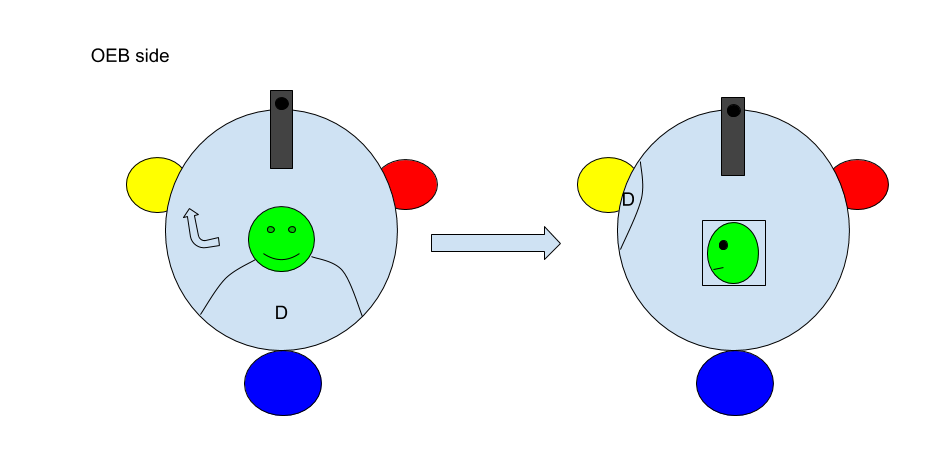
\includegraphics[scale=0.6]{fig/PCimgSlideYoko.png}
  \caption{OmniEyeBall上で,PC使用者の表示位置が移動する模式図}
\end{figure}
\end{comment}

6-2-1で会話中のビデオ会議参加者を表示する方法を提案した.本節では
立体的な映像を表示するという部分に着目し,小窓に横顔を
表示する方法を提案する.

\begin{figure}[tp]
  \centering
  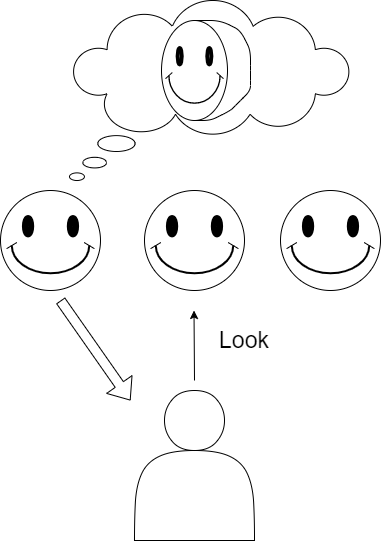
\includegraphics[scale=0.7]{fig/yokogao.png}
  \caption{横顔が見える状況} \label{yokogao}
\end{figure}

表\ref{yokogao}のように,複数人で対面している状況を考える.
話者が自身に話しかけていない場合,別の人物に顔を向けている
場合が多く,その際には話者の横顔が視認できる.
ここでは,小窓に話者の正面顔ではなく横顔を表示する
方法を提案する.対面時の立体的情報を再現することで,
ビデオ会議の参加者に更なる没入感を提供することが目的である.

実装時間の関係で,参加者の実際の顔の横顔を再現するには至らなかった.
このことは今後の課題とする.代用案として,昨今様々な場所で配布されており,
入手・仕様・作成が容易な3Dモデルを利用して,横顔を表示する手法を提案する.

3Dモデルの撮影にはUnity\cite{16}を用いた.UnityではOpenCV及びDlib
が利用可能で,Dlibで取得した顔のランドマーク情報から3Dモデルの体や表情を
動かすことが可能である.また,Unityでは自由にシーン描画カメラを配置することができる,
ここでは3Dモデルの左右にカメラを配置し,リアルタイムで横顔を撮影した.
Unity内カメラの映像はUnityCapture\cite{8}を利用することで,容易に
仮想カメラの映像として利用することが出来る.

\begin{figure}[tp]
  \centering
  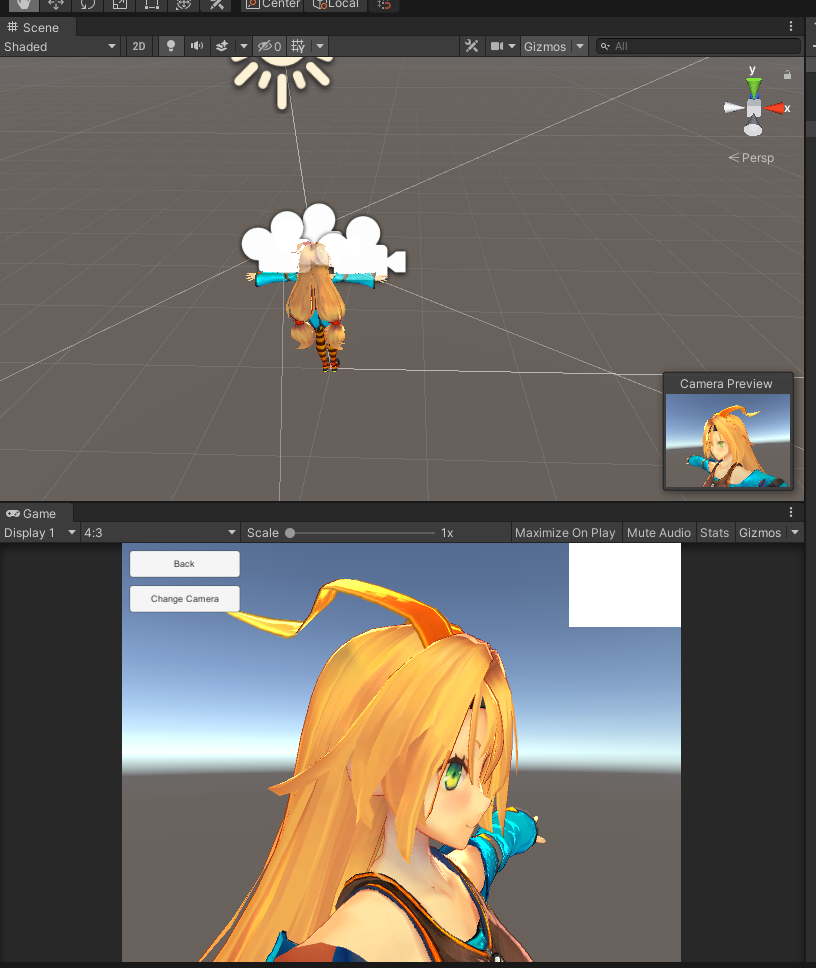
\includegraphics[scale=0.7]{fig/unitycam.png}
  \caption{3Dモデルを撮影する様子}
\end{figure}

\begin{figure}[tp]
  \centering
  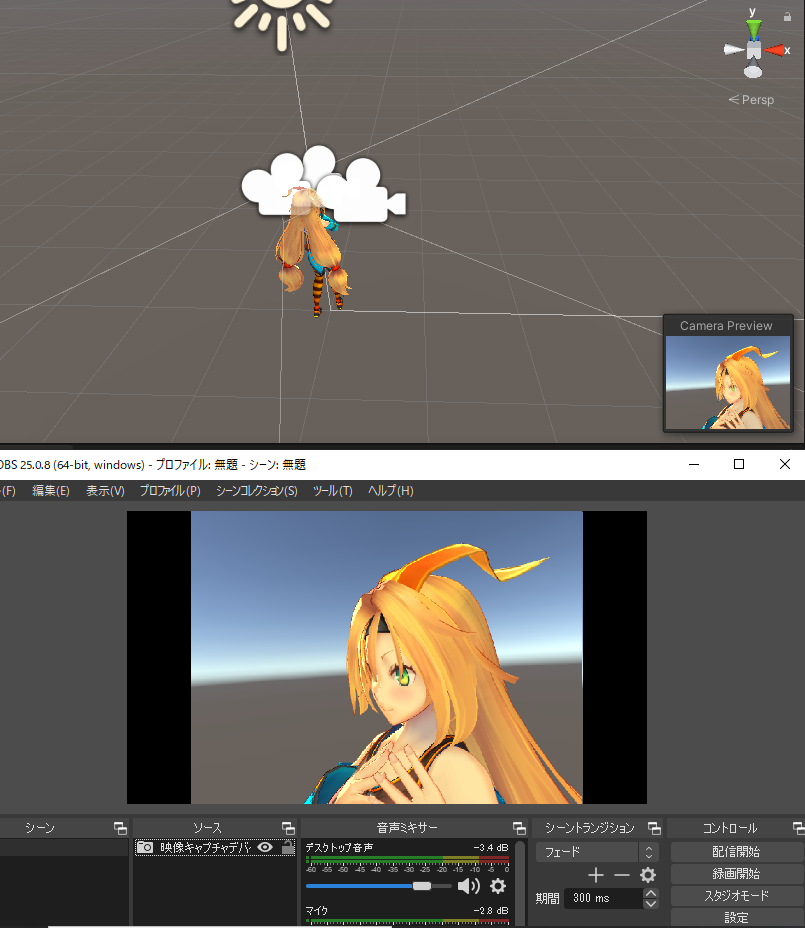
\includegraphics[scale=0.6]{fig/unitycapture.png}
  \caption{UnityCaptureを用いた他アプリケーションへの映像ストリーミング}
\end{figure}

通信の高速化のため,プロセス間通信で顔の位置情報を送信し,カメラを移動させる
ということは行わなかった.OmniEyeBallの使用者から見て,右側の参加者が見られているときには
左から見た横顔が,左側の参加者が見られているときには右から見た横顔が表示されるようにした.

\begin{figure}[tp]
  \centering
  \includegraphics[scale=0.2]{fig/yokoV.png}
  \caption{生成した横顔をOmniEyeBall上で表示させた様子}
\end{figure}

今後,ビデオ会議参加者自身の顔を生成する方法としては,
後述するおかしら会議\cite{10}の表示法を用いる手段がある.
Unity内の仮想球体にspriteとして,PC使用者の顔写真を張り付ける.
そうした球体を撮影することで,疑似的な顔写真を生成する.

機械学習ベースの方法として,横顔生成手法としてYiboら\cite{11}の方法が挙げられる.
これらの方法を用いた表示は,今後の研究課題とする.
  \subsection{おかしら会議形式}\begin{comment}
\begin{itemize}
  \item 全天球映像の表示方法自体を変更する手段として,宮藤ら\cite{10}のおかしら会議が挙げられる
  \item 球体ディスプレイそのものを顔として見立て,全天球映像の顔部分のみをマッピングする
  \item マッピングする際に,全天球パノラマ画像上下部分に見られる歪みを考慮し,修正する式を用いている
  \item (式を乗せて,どのように歪み補正が行われているかを説明)
  \item (アプリケーションが動いている様子も載せる)
\end{itemize}
\end{comment}

全天球映像の表示方法自体を変更する手段として,宮藤ら\cite{10}のおかしら会議が挙げられる.
これは球体ディスプレイそのものを顔として見立て,全天球映像の顔部分のみをマッピングするという手法である.

顔の切り抜きは,Dlibを用いて検出された顔バウンディングボックスによって行い,
拡大したのちに楕円形にトリミングする.その画像を背景が黒い長方形画像に張り付け,
正距方位図法への変換を行う.

この際,長方形にそのまま楕円顔画像を張り付けてしまうと,上下部分がが
相対的に小さく描画されてしまう.よって,その歪みを打ち消す処理を行っている.

\begin{figure}[tp]
  \centering
  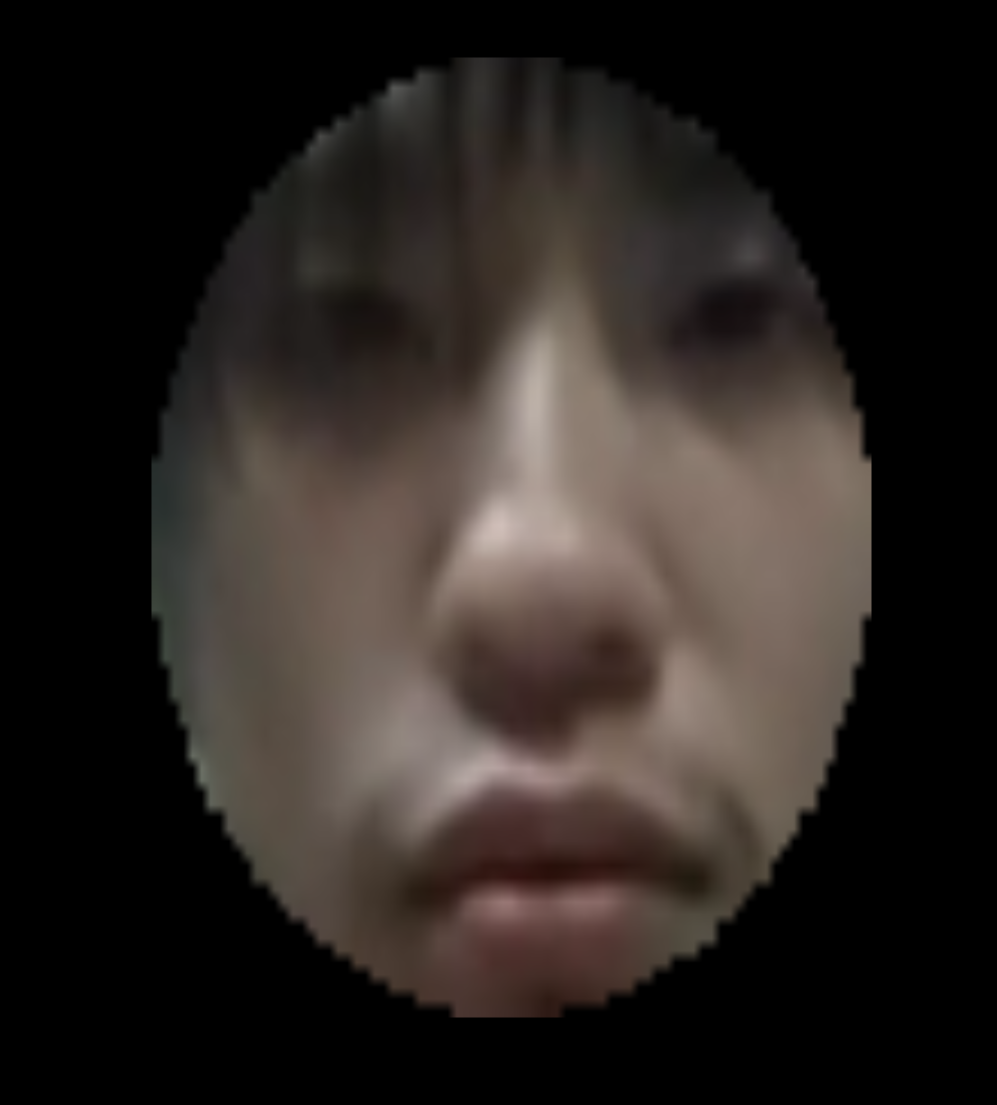
\includegraphics[scale=0.6]{fig/okashira1.png}
  \includegraphics[scale=0.15]{fig/okashira3.png}
  \caption{歪みの補正前}
\end{figure}

\begin{figure}[tp]
  \centering
  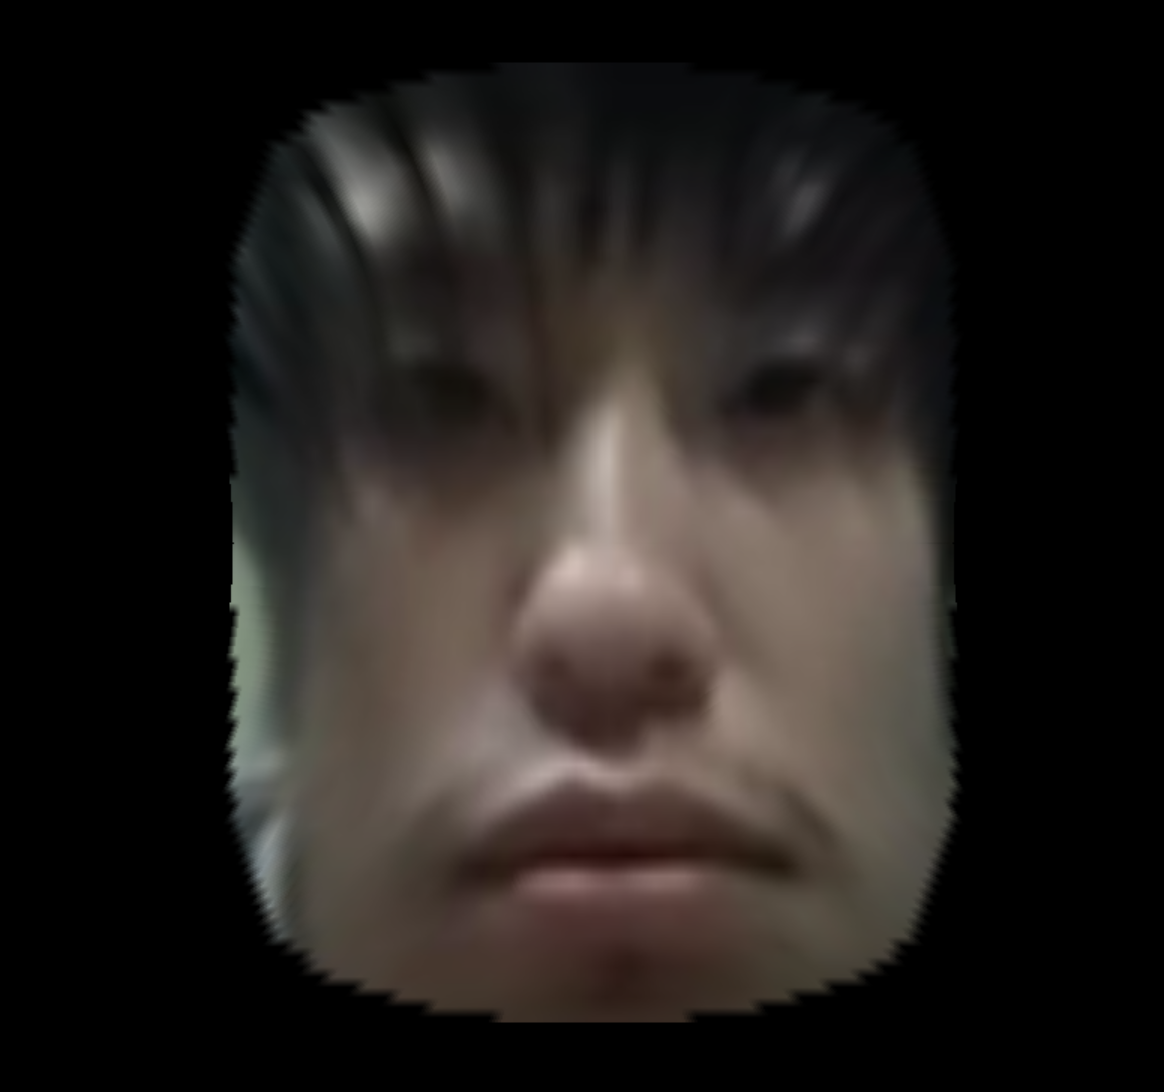
\includegraphics[scale=0.6]{fig/okashira2.png}
  \includegraphics[scale=0.15]{fig/okashira4.png}
  \caption{歪みの補正後}
\end{figure}

実験の考察でも述べた通り,立体的な資格情報は,
ビデオ会議での疑似的な対面経験を作り出すとみられる.
よって現実の顔に近い立体表現が可能なこの表示方法は
効果的であると考えられる.

問題点としては,全天球画像の顔の領域が小さいことが挙げられる.
小さい画像を拡大して大きな画像に張り付けるため,画質が著しく低下してしまう.

しかし,近年は4K画質に対応したカメラが多く存在し,全天球カメラにも
4K画質のものが存在する.GPUの性能向上と合わせ,高解像度のカメラ映像を遅延なく
送信することができれば,この問題は解決される.
\section{今後の展望}\begin{comment}
\begin{itemize}
  \item 6-2で,様々な顔の表示方法を提案した.
  \item コロナ禍の影響で十分な実験を行うことが出来なかった
  \item 提案したアプリケーションを用いて,十分な実験を行い,比較を行うことで,
  最適な表示方法を決定することが今後の課題である
  \item 一方で解決できていない問題も存在する
  \item 小窓が表示される際に,突然表示されて使用者が驚いてしまう
  \item 複数の人間に話しかけている場合の顔や小窓の表示方法
  \item 今後の研究でそれらの問題を解決する方法を模索していく
  \item また,今回のアプリケーションは個人対複数人といったユースケースに限られている
  \item 個人の参加者が複数人いた場合,OmniEyeBall上での表示をどのようにするかという問題がある.
  \item 例えば,OmniEyeBall側で,現在映したい人物を選択できるようにすれば,今回のシステムをそのまま活用できる
  \item 一方で,会話にPC使用者が複数人参加している場合には,同時に映すことが出来ない
  \item このようなユースケースにも対応していく方法も検討する必要がある
\end{itemize}
\end{comment}
本章では,5章で得られた知見に基づいていくつかのアプリケーションを
提案してきたが,依然解決できていない問題がある.

\subsubsection*{特定の一人を見ていないケース}
アンケート結果によって,小窓を既に表示されている顔の上に表示するのは
混乱を招いている可能性があると結論付けた.よって提案したアプリケーションでは
その表示方法を廃止した.しかし,先の表示方法は,実験用アプリケーションで特定の一人を見ていないケース
を区別していた表示方法であった.この状況を表す代替の表示方法を提示する必要がある.

案の一つとしては,テキストや印を表示する方法がある.
しかし,小さいとサインが見えにくく,大きすぎると
映像の邪魔になってしまう.なおかつ,本アプリケーションは
従来の方法に比べ,SUSの評価が向上したとは言えず,これ以上の
情報提示は,ただでさえ複雑なアプリケーションをさらに複雑にすると
考え,実装を見送った.

\subsubsection*{全天球ビデオカメラの回転の問題}

本アプリケーションは,使用開始前の
状態として,PCの使用者が全天球パノラマ画像の
中心部を見ている前提で,画像のスライドや顔認識した位置に
画像を張り付ける処理を行ってきた.しかし,カメラが回転すると,
基準としていた位置がずれ,ずらす処理にも変更を加える必要がある.
だが,本研究では回転を考慮した処理を行っていない.

これを解決する案として,特徴点マッチングを用いる方法が考えられる.
特徴点マッチングによって,画像のスライド距離を算出し,その値を
本論文の処理に加えて反映させれば,この問題は解決できるであろう.

\begin{figure}[tp]
  \centering
  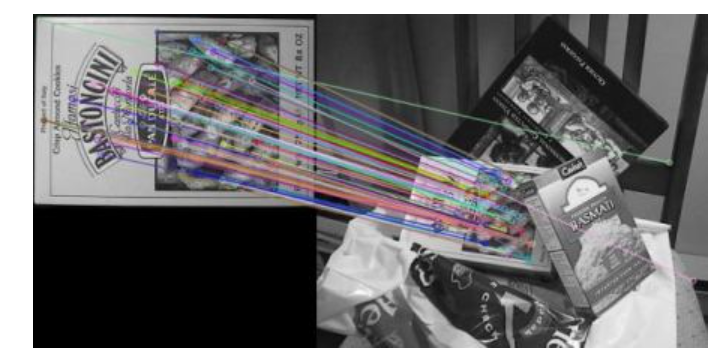
\includegraphics[scale=0.7]{fig/matching.png}
  \caption{特徴点マッチング} \cite{17}
\end{figure}

\subsection*{視線認識の導入}
実験で用いたアプリケーションのSUSの評価が
従来のビデオ会議アプリケーションより悪化した項目も
多かった原因として,従来のビデオ会議にはなかったクリック操作
の存在が可能性として挙げられる.また,PC使用者のコメントで
「常に全員が視界に入っていた」というものがあったように,視野の広さのせいで
PC使用者が,見るという動作を重要視しない恐れがある.
これを解決する方法として,Tobii Eye tracker\cite{30}等の
画面上の視線認識器具の利用が考えられる.

\subsubsection*{様々なケースへの対応}
今回は個人対複数人でのビデオ会議という状況
を前提において研究を進めてきた.しかし実際には
他にも以下のようなケースが存在する.
\begin{itemize}
  \item 複数のOmniEyeBallを使用するケース
  \item OmniEyeBallから孤立した参加者が複数人であるケース
  \item 孤立した参加者の何人かが共通の空間にいるケース
\end{itemize}

例えば2番目のケースは,OmniEyeBall側の参加者が現時点で注目したい
遠隔参加者を1人選ぶというようにする.さすれば,その1人に対して
今回提案したシステムが利用可能である.

しかし1番目のケース,3番目のケースは,複数人が同じ空間を
共有している.今回のような画像の回転を用いると,意図していない人物の
回転を同時に招いてしまう.これらの複雑なケースに沿ったシステムを
提案していくことは,今後の研究課題である.

\subsubsection*{まとめ}
今後の研究方針としては,先に述べたような
複雑なケースに対応するシステムの模索が考えられる.
一方,今回はコロナ禍の影響で,十分に実験が行えたとは言えない.
十分な時間を要して,今回提案した複数の表示方法について
綿密な実験を繰り返し,より多くのユーザーの実体験に
基づいた知見を獲得していくことも必要であろう.


%%%%%%%%%%%%%%%%%%%%%%%%%%%%%%%%%%%%%%%%%%%%%%%%%%

\chapter{結論}
結論は、網羅的にかつ簡潔に。

%%%%%%%%%%%%%%%%%%%%%%%%%%%%%%%%%%%%%%%%%%%%%%%%%%


%\appendix
%\chapter{定理1の証明}
%必要に応じて、付録を載せる。

%%%%%%%%%%%%%%%%%%%%%%%%%%%%%%%%%%%%%%%%%%%%%%%%%%

\backmatter
\chapter{謝辞}
本論文の執筆にあたり、議論して頂いた関係者に感謝する.

%%%%%%%%%%%%%%%%%%%%%%%%%%%%%%%%%%%%%%%%%%%%%%%%%%

\bibliographystyle{jplain}
\bibliography{references}
\begin{thebibliography}{99}
%  \bibitem{tokodai-xyz2015} 東工大太郎. 良い論文の書き方. \textit{Journal of XYZ}, Vol.~3, No.~4, pp. 15--34, 2015.
  
\bibitem{1}zoomの説明
\bibitem{2}google meetの説明
\bibitem{3}The GAZE groupware system: mediating joint attention in multiparty communication and collaborationの文献
\bibitem{4}Theta Vの説明(https://theta360.com/ja/about/theta/)
\bibitem{5}Collaboration in 360° Videochat: Challenges and Opportunitiesの文献
\bibitem{6}Can You See Me Now?: How Field of View Affects Collaboration in Robotic Telepresenceの文献
\bibitem{7}OBS-virtual-camの説明
\bibitem{8}UnityCaptureの説明(https://github.com/schellingb/UnityCapture)
\bibitem{9}OEBStudioの説明
\bibitem{10}おかしら会議の文献
\bibitem{11}Pose-Guided Photorealistic Face Rotationの文献
\bibitem{12}Dlibの説明(http://dlib.net/)
\bibitem{13}https://ci.nii.ac.jp/naid/40021907210
\bibitem{14}%https://www.jstage.jst.go.jp/article/hozen/advpub/0/advpub_1822/_pdf/-char/ja
\bibitem{15}glomal 350の説明(https://www.aisan.co.jp/products/glomal350.html)
\bibitem{16}Unity https://unity.com/ja
\bibitem{17}有志によるOpenCVの解説(http://labs.eecs.tottori-u.ac.jp/sd/Member/oyamada/OpenCV/html/py\_tutorials/py\_feature2d/py\_matcher/py\_matcher.html)
\bibitem{18}OmniEyeBall(https://dl.acm.org/doi/10.1145/3266037.3266092)
\bibitem{19}Collaboration in 360° Videochat: Challenges and Opportunities
\bibitem{20}%https://ja.wikipedia.org/wiki/%E3%83%86%E3%82%A4%E3%82%BD%E3%83%BC%E3%81%AE%E6%8C%87%E7%A4%BA%E6%A5%95%E5%86%86#/media/%E3%83%95%E3%82%A1%E3%82%A4%E3%83%AB:Tissot_indicatrix_world_map_equirectangular_proj.svg
\bibitem{21}Meeting OWL(http://meetingowl.jp/?i=nav)
\bibitem{22}WORLDEYE
\bibitem{23}iSphere: Self-Luminous Spherical Drone Display
\bibitem{24}How Display Shapes Affect 360-Degree Panoramic Video Communication
\bibitem{25}An Interactive Omnidirectional Ball Display
\bibitem{26}Comparing flat and spherical displays in a trust scenario in avatar-mediated interaction
\bibitem{27}Room2Room: Enabling Life-Size Telepresence in a Projected Augmented Reality Environment
\bibitem{28}Improving Visibility of Remote Gestures in Distributed Tabletop Collaboration
\bibitem{29}A Gaze-preserving Group Video Conference System using Screen-embedded Cameras
\bibitem{30}https://www.tobiipro.com/ja/product-listing/
\bibitem{31}OmniView: An Exploratory Study of 360 Degree Vision using Dynamic Distortion based on Direction of Interestの文献
\bibitem{32}cubemapの説明(https://docs.unity3d.com/ja/2018.4/Manual/class-Cubemap.html)
(後で正式な書式に書き直します)

\end{thebibliography}

\end{document}
